\documentclass[11pt, a4paper, twoside, openright]{book} 
\usepackage[italian, english]{babel}
\usepackage[sc]{mathpazo}
\usepackage[utf8]{inputenc}
\usepackage{setspace}
\onehalfspacing	
\usepackage{microtype}
\usepackage[inner=4cm, outer=3cm, top=3cm, bottom=3cm]{geometry}
\usepackage{graphicx}
\graphicspath{ {./img/} }
\usepackage{tabularx}
\usepackage{booktabs}
\usepackage[hang, small,labelfont=bf,up,textfont=it,up]{caption}
\usepackage[Bjornstrup]{fncychap}
\ChNumVar{\fontsize{76}{80}\usefont{OT1}{pzc}{m}{n}\selectfont\color{black}}  
\ChTitleVar{\raggedleft\LARGE\bfseries}
\usepackage{epigraph}
\usepackage{xcolor}
\usepackage{multicol}
\usepackage{pdfpages}
\usepackage[pdftex]{hyperref}
\hypersetup{
	bookmarksnumbered,	% Chapter and Appendix Numbers
	colorlinks,
	citecolor=black,
	filecolor=black,
	linkcolor=black,
	urlcolor=black
}
\usepackage{listings}
\usepackage{multicol}

\definecolor{backcolour}{RGB}{255,255,255}
\definecolor{codegreen}{RGB}{27,168,11}
\definecolor{codeblue}{RGB}{35,35,205}
\definecolor{codegray}{RGB}{128,128,128}
\definecolor{codepurple}{RGB}{205,35,56}
\lstdefinestyle{myPython}{
	backgroundcolor=\color{backcolour},   
	commentstyle=\color{codegreen},
	keywordstyle=\color{codeblue},
	numberstyle=\tiny\color{codegray},
	stringstyle=\color{codepurple},
	basicstyle=\small\ttfamily,
	breakatwhitespace=false,         
	breaklines=true,                 
	captionpos=b,                    
	keepspaces=true,                 
	numbers=left,                    
	numbersep=5pt,                  
	showspaces=false,                
	showstringspaces=false,
	showtabs=false,                  
	tabsize=2,
	language=python
}

\usepackage[titletoc]{appendix}

\usepackage{tabularx}

\title{Tesi Triennale}
\author{FEDERICO MATTEONI}
\date{Giugno-Agosto 2021}

\begin{document}
	\selectlanguage{italian} 
	
	\frontmatter
	% Il frontespizio viene importato da un file pdf con una singola pagina
	\begin{titlepage}
		\thispagestyle{empty}
		
\includepdf{frontespizio/frontespizio.pdf}
		\thispagestyle{empty}
		\cleardoublepage
	\end{titlepage}	
	%\null \vspace{\stretch{1}}
\begin{flushright}
\textit{Dedica per qualcuno}
\end{flushright}
\vspace{\stretch{2}} \null \cleardoublepage
	\cleardoublepage
	\phantomsection
	\pdfbookmark{\contentsname}{tableofcontents}
	\tableofcontents
	\cleardoublepage
	\phantomsection
	\addcontentsline{toc}{chapter}{Immagini}
	\listoffigures
	\cleardoublepage
	\phantomsection
	\addcontentsline{toc}{chapter}{Tabelle}
	\listoftables
	\phantomsection
\chapter*{Glossario}
\markboth{GLOSSARIO}{}
\addcontentsline{toc}{chapter}{Glossario}

\subsection*{Abbreviazioni e Acronimi}
\begin{table}[h!]
	\begin{center}
		\begin{tabularx}{\textwidth}{ll}
			\toprule
			\textsc{Termine} & \textsc{Significato} \\ 
			ML & Machine Learning\\
			HSM & Human State Monitoring, Monitoraggio dello Stato Umano\\
			ReLU & Rectified Linear Unit, Unità Lineare Rettificata\\
			RNN & Recurrent Neural Network, Rete Neurale Ricorrente\\
			LSTM & Long Short-Term Memory, Memorie a Lungo Breve-Termine\\
			LWF & Learning Without Forgetting, Apprendere Senza Dimenticare\\
			EWC & Elastic Weight Consolidation, Consolidamento Elastico dei Pesi\\
			FWT & Forward Transfer, Trasferimento in Avanti\\
			BWT & Backward Transfer, Traserimento all'Indietro\\
			HAR & Human Activity Recognition\\
			MNIST & Modified National Institute of Standards and Technology Database\\
			GRU & Gated Recurrent Unit, Unità Ricorrente con Cancello\\  % intraducibile
			GPU & Graphics Processing Unit, Unità di Processo Grafico\\
			TPU & Tensor Processing Unit, Unità di Processo Tensoriale\\
		\end{tabularx}
	\end{center}
\end{table}
	\phantomsection
\chapter*{Introduzione}
\markboth{INTRODUZIONE}{}
\addcontentsline{toc}{chapter}{Introduzione}

Negli ultimi decenni, l'"Intelligenza Artificiale" se è fatta sempre più spazio nella nostra vita di tutti i giorni. Grazie ai nostri smartphone, usiamo modelli di Machine Learning efficienti che indirizzano le nostre ricerche nella rete, e grazie a tali modelli le aziende possono mostrarci inserzioni sempre più aderenti ai nostri gusti personali. Ma il mondo del Machine Learning ha importanti e utili applicazioni anche nella salvaguardia del benessere dell'individuo, ad esempio in contesti come il riconoscimento delle malattie o l'interpretazione del linguaggio parlato. Questi contesti, che rientrano nell'ambito dello \textit{Human State Monitoring}, stanno diventando sempre più importanti nella vita di tutti i giorni e diventerà sempre più necessario l'avere a disposizione sistemi che sappiano sfruttare efficacemente i dati sull'utente che hanno a disposizione, così da realizzare sistemi responsivi e reattivi in base allo stato attuale dell'utente.\\\\
Con Addestramento Continuo si definisce l'approccio all'addestrare un modello di Machine Learning in diverse sessioni di addestramento distribuite nel tempo, con l'obiettivo di migliorare gradualmente la sua performance. Questo approccio può portare ad un graduale deterioramento delle conoscenze acquisite nelle sessioni di addestramento iniziali: la nuova conoscenza può soppiantare la conoscenza già appresa, e questo fenomeno prende il nome di \textit{catastrophic forgetting}. Attualmente, diversi studi concentrano i propri sforzi sul risolvere alcune problematiche intrinseche nell'Addestramento Continuo, come il \textit{catastrophic forgetting}$^{\cite{kirkpatrick2017overcoming},\cite{li2017learning},\cite{DBLP:journals/corr/Lopez-PazR17},\cite{rolnick2019experience}}$ o riguardanti la realizzazione in contesti reali di produzione di infrastrutture di continual learning$^{\cite{diethe2019continual}}$, mentre ulteriori studi hanno analizzato l'applicabilità in altri contesti come la \textit{Human Activity Recognition}$^{\cite{Jha_2021}}$ o l'acquisizione di informazioni dai social network$^{\cite{priyanshu2021continual}}$. Sono rari gli studi sullo \textit{Human State Monitoring} e ancora non è stato realizzato un confronto fra le tecniche di Addestramento Continuo di questa tesi.\\
L'obiettivo è dunque mettere a confronto alcune metodologie di Addestramento Continuo su dati relativi allo \textit{Human State Monitoring}.
\subsection*{Obiettivi}
L'obiettivo principale di questa tesi è studiare, attraverso una serie di esperimenti, le performance raggiunte da alcune metodologie di Apprendimento Automatico Continuo applicate a Reti Neurali Ricorrenti riguardo problemi che rientrano nell'ambito dello \textit{Human State Monitoring}. Per poter realizzare questo obiettivo sono stati individuati alcuni sotto-obiettivi necessari alla realizzazione degli esperimenti e della comparazione.
\begin{itemize}
    \item[-] \textbf{Individuare dataset contenenti dati realitivi allo \textit{Human State Monitoring}}\\
    Per poter valutare la sinergia tra continual learning e \textit{Human State Monitoring}, inanzitutto si rende necessaria la raccolta di dati riguardanti lo HSM. Ne sono stati individuati due, scelti per le caratteristiche che verranno discusse in seguito: WESAD$^{\cite{10.1145/3242969.3242985}}$ e ASCERTAIN$^{\cite{7736040}}$.
    \item[-] \textbf{Selezionare le metriche e le informazioni utili alla comparazione delle varie metodologie}\\
    Comparare le varie metodologie significa avere a disposizione per ognuna di esse delle metriche che vadano a misurare i loro vari aspetti, come il tempo necessario all'addestramento, l'accuratezza raggiunta, la conoscenza trasferita e l'impatto a livello di memoria.
    \item[-] \textbf{Scegliere una \textit{baseline}}\\
    Cioè una metodologia base da cui partire e che sia utile a confrontare tutti gli altri. Come sarà specificato in seguito, la metodologia scelta come baseline sarà quella \textit{offline}: ciò consiste nell'addestramento di una rete neurale usando l'intero training set a disposizione senza usare approcci continual.
    \item[-] \textbf{Definire gli strumenti tecnologici}\\
    Si rende necessario individuare un ambiente in cui poter eseguire le computazioni necessarie all'addestramento, identificare le API e i linguaggi di programmazione adatti allo scopo e produrre del codice verificabile e degli esperimenti replicabili.
    \item[-] \textbf{Confrontare i risultati e trarre le conclusioni}\\
    Una volta raccolti tutti i dati necessari, essi verranno confrontati per poter finalmente valutare la sinergia fra continual learning e Human State Monitoring.
\end{itemize}
\pagebreak
\subsection*{Risultati}
Gli esperimenti e i risultati prodotti nell'ambito di questa tesi mostreranno quanto le tecniche di Addestramento Continuo siano applicabili a contesti di \textit{Human State Monitoring} con risultati anche comparabili all'apprendimento classico \textit{offline}. In particolare, molte delle tecniche di addestramento continuo adottate riescono a ottenere risultati inferiori ma comunque buoni quando applicate alla medesima struttura di rete neurale utilizzata nell'addestramento offline, con misure di trasferimento della conoscenza spesso anche molto positive.

\subsection*{TEACHING}
Questa tesi è stata svolta nell'ambito del progetto TEACHING$^{\cite{teaching2020}}$.\\TEACHING è un progetto finanziato dall'Unione Europea volto a progettare una piattaforma informatica ed il relativo toolkit software a supporto dello sviluppo e del rilascio di applicazioni autonome, adattive e affidabili, consentendo a tali applicazioni di sfruttare il feedback umano per guidare, ottimizzare e personalizzare i servizi offerti.

\subsection*{Struttura della tesi}
Nel capitolo 1 verranno definite nel dettaglio le conoscenze preliminari necessarie per affrontare gli argomenti di questa tesi. Nei due capitoli successivi verranno presentati, rispettivamente, le due raccolte di dati utilizzate negli esperimenti (capitolo 2) e gli approcci di addestramento continuo messe a confronto (capitolo 3).
Nel capitolo 4 vengono presentati nel dettaglio i risultati prodotti nell'ambito della tesi. Infine, nel capitolo 5, sono delineate le conclusioni tratte a partire da tali risultati.
    
    \mainmatter
    \chapter{Preliminari}
In questo capitolo verranno presentati alcuni degli argomenti preliminari necessari alla realizzazione della tesi.\\
Nella sezione 1.1 viene presentato il contesto riguardante l'ambito del Machine Learning, presentando gli argomenti di questo campo di studi che riguardano questa tesi. Nella sezione 1.2 si presenta l'attuale stato dell'arte riguardo le Reti Neurali Ricorrenti, gli strumenti a disposizione e alcune future possibili applicazioni degli argomenti trattati in questa tesi.

\section{Contesto}
In un mondo sempre più interconnesso e in rapida evoluzione, gli approcci statici al Machine Learning possono diventare impraticabili quando si tratta di produrre sistemi in grado di adattarsi dinamicamente allo stato fisico e mentale degli utenti che vi interagiscono. Inoltre, con l'ampia diffusione di dispositivi in grado di raccogliere in tempo reale informazioni sulla condizione attuale degli utenti, sono costantemente resi a disposizione nuovi dati con cui perfezionare i modelli di Machine Learning in uso attraverso tecniche di addestramento continuo.

\subsection{Human State Monitoring}
Uno di questi contesti è lo \textit{Human State Monitoring}. Con questo termine si indica l'obiettivo di un sistema di raccogliere dati riguardanti l'attuale stato psico-fisico di un individuo e trarre conclusioni sulla sua condizione attuale, ad esempio interpretando un battito cardiaco elevato insieme ad un alto livello di sudorazione come uno stato di stress, o determinati movimenti facciali come una condizione di sonnolenza. L'avere a disposizione metodologie efficienti nel catalogare queste condizioni umane può portare a sistemi responsivi e adattivi, che modificano le proprie interfacce o i propri comportamenti accomodando lo stato psico-fisico attuale dell'utente.\\\\
Un possibile applicazione dello \textit{Human State Monitoring} la si può trovare nel progetto europeo TEACHING$^{\cite{teaching2020}}$, che mira alla produzione di un toolkit per costruire applicazioni autonome efficienti che facciano uso di intelligenza simile a quella umana. L'obiettivo di questo toolkit è supportare lo sviluppo e il rilascio di applicazioni che possano sfruttare il feedback umano per ottimizzare, personalizzare e guidare il modo in cui esse forniscono i propri servizi. In altre parole, applicazioni che sfruttino lo \textit{Human State Monitoring} per adattarsi dinamicamente alle condizioni dell'utente in tempo reale.\\
Per poter realizzare questo adattamento continuo è necessario, oltre al flusso di dati in tempo reale sullo stato corrente dell'utente, anche un sistema che sappia efficientemente e correttamente interpretare questi dati, traendo conclusioni sulle attuali condizioni della persona. Questa situazione presenta le classiche caratteristiche necessarie all'applicazione del Machine Learning: abbiamo dati raccolti da sensori che possono essere difettosi, per cui i dati possono contenere incertezze o essere rumorosi o incompleti, ed essendo in esame lo stato umano è molto difficile, se non impossibile, formalizzare attraverso una descrizione procedurale la classificazione di questi dati in categorie comportamentali, ad esempio affaticamento o sonnolenza.

% breve introduzione al mondo dell'addestramento Machine Learning per introdurre i concetti fondamentali per la tesi
\subsection{Addestramento} L'addestramento di un modello di Machine Learning avviene attraverso l'utilizzo di un insieme di dati chiamato \textit{training set}, che contiene i dati di addestramento. Questi dati sono sottoposti al modello, che li userà nelle sessioni di addestramento. Nell'addestramento supervisionato, il training set è composto da una serie di esempi composti da coppie $\langle$input, etichetta$\rangle$ dove le etichette sono fornite da chi ha preparato il training set, detto supervisore. Queste etichette vengono assegnate agli input in base ad una certa funzione $f$, che è ignota ed è la funzione che il modello di Machine Learning deve apprendere. Il modello elabora questi dati e le loro etichette cercando di apprendere quali etichette sono assegnate a quali dati e in che modo. L'obiettivo del modello è quindi trovare una buona approssimazione di $f$ che faccia corrispondere le etichette corrette ai rispettivi input.\\
Per verificare l'apprendimento, si sottopone al modello addestrato dei dati non etichettati, denominati \textit{test set}, e si verificano le etichette che il modello assegna a tali dati controllando se ha classificato correttamente o meno. La percentuale di dati correttamente etichettati dal modello è chiamata \textbf{accuratezza}.

\subsection{Loss} Per misurare l'andamento dell'apprendimento di un modello di Machine Learning, vengono usate funzioni che vanno a valutare il modello in base alle risposte che esso fornisce sui dati etichettati, confrontandole con le etichette reali. Queste funzioni prendono il nome di funzioni di \textit{loss}. Ne esistono di diversi tipi, a seconda del problema in esame: ad esempio, nei problemi dove ad ogni input va assegnata una risposta si/no (classificazione binaria) una loss molto usata è la cross-entropia binaria (\textit{binary crossentropy}), delineata nell'equazione \ref{eq:bin_crossentr} dove $y$ è l'etichetta reale, che può assumere valori 0/1, falso/vero o altri, e $p(y)$ è la probabilità assegnata dal modello in fase di previsione.
\begin{equation}\label{eq:bin_crossentr}
H_p(q) = -\frac{1}{N}\sum_{i=1}^N \left(y_i\cdot\log(p(y_i)) + (1 - y_i)\cdot\log(1 - p(y_i))\right)
\end{equation}

\subsection{Reti Neurali} In letteratura vengono studiati moltissimi modelli di Machine Learning. Si va dai più semplici come i modelli lineari, nei quali abbiamo un'equazione nella forma $y = w_0x + w_1$ e dobbiamo apprendere i $w_0$ e $w_1$ che ai dati $x$ fanno corrispondere le corrette etichette $y$, alle \textit{Support Vector Machine}, che cercano di trovare dei confini di divisione fra insiemi di dati così da poterli classificare.\\
Un'ampia area di modelli di Machine Learning è quella delle cosiddette \textbf{reti neurali}, studiate sin dagli anni '40. Esse prendono liberamente spunto dalla struttura dei neuroni del cervello umano (Figura \ref{fig:neurone}), che sono stati schematizzati in strutture matematiche denominate \textbf{perceptron}$^{\cite{rosenblatt1958perceptron}}$.
\begin{figure}[h]
	\begin{center}
		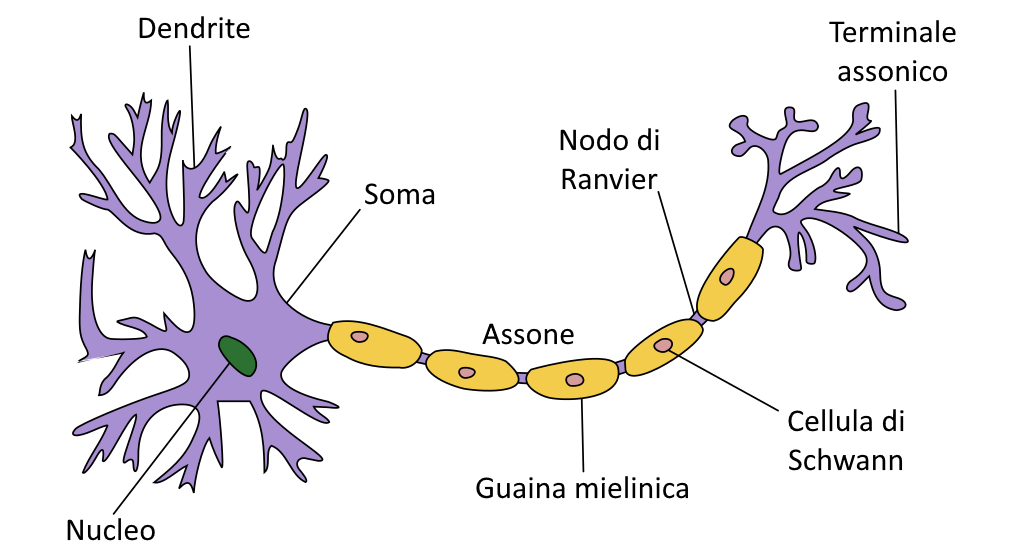
\includegraphics[width=0.75\textwidth]{img/neurone.png}
		\caption{Neurone (credits: Quasar, Wikipedia)}
		\label{fig:neurone}
	\end{center}
\end{figure}
In un perceptron (Figura \ref{fig:perceptron}), ad ogni input $x_i$ è assegnato un peso $w_i$ che lo rende più o meno importante nel contribuire al risultato $y$, che viene calcolato dal nodo attraverso la \textbf{funzione di attivazione}, nella forma \ref{eq:act_fun} dove $b$ è un ulteriore peso definito \textit{bias}.\\\\
\begin{equation}\label{eq:act_fun}
f\left(\sum_i w_i\cdot x_i + b\right)
\end{equation}
\begin{figure}[h]
	\begin{center}
		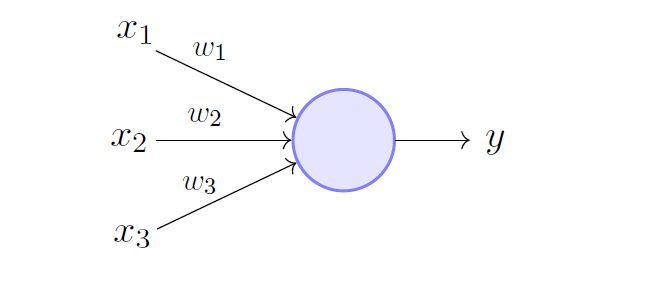
\includegraphics[width=0.5\textwidth]{img/perceptron.png}
		\caption{Perceptron}
		\label{fig:perceptron}
	\end{center}
\end{figure}
Una rete neurale (Figura \ref{fig:reteneurale}) è composta da un insieme di perceptron collegati fra loro suddivisi su livelli, o \textit{layer}: una rete neurale composta da un elevato numero di layer è detta profonda, o \textit{deep neural network}, e i layer interni sono detti layer nascosti.
\begin{figure}[h]
	\begin{center}
		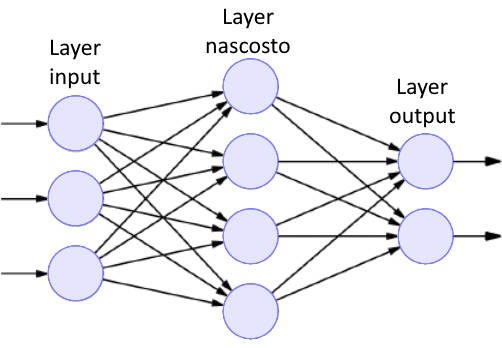
\includegraphics[width=0.75\textwidth]{img/reteneurale.jpg}
		\caption{Esempio di rete neurale (credits: databricks.com)}
		\label{fig:reteneurale}
	\end{center}
\end{figure}
\\\\
Le funzioni di attivazione possono essere funzioni di qualsiasi tipo, ma le più usate e studiate sono funzioni specifiche come ReLU e softmax. La funzione ReLU (\textit{Rectified Linear Unit}) è molto semplice e veloce da calcolare: restituisce la parte positiva del proprio input, e consente un migliore apprendimento nelle reti neurali profonde$^{\cite{pmlr-v15-glorot11a}}$.
\begin{equation}\label{eq:fun_relu}
ReLU(x) = max(0, x)
\end{equation}
La funzione softmax, invece, prende in input un vettore di $K$ valori e lo comprime in un vettore sempre di $K$ elementi ma dai valori compresi nell'intervallo $(0, 1)$ e la cui somma è 1. Vengono usate nel layer finale delle reti neurali realizzate per compiti di classificazione: ogni valore $\sigma(\textbf{z})_j$  è interpretabile come la probabilità che l'input appartenga alla classe $j$ fra le $K$ possibili.
\begin{equation}\label{eq:fun_softmax}
\sigma(\textbf{z})_j = \frac{e^{z_j}}{\sum_{k=1}^K e^{z_k}}\:\:\:\:\mbox{ per }j = 1,\ldots,K
\end{equation}
Le funzioni di attivazione descrivono quindi il comportamento dei nodi di una rete neurale e la scelta della funzione di attivazione è un elemento importante nella strutturazione di una rete neurale.
\subsubsection{Tipologie} La struttura interna di una rete neurale influenza particolarmente i risultati che essa può ottenere. A seconda del problema che si vuole risolvere, si può rendere necessario l'utilizzo di reti neurali con strutture interne complesse, in modo da ottenere risultati soddisfacenti. In particolare, in letteratura attualmente alcune delle strutture più studiate sono (Figura \ref{fig:tipologiereti}):
\begin{itemize}
    \item[-] Reti Feed Forward (FF)$^{\cite{0471349119}}$
    \item[-] Reti Neurali Ricorrenti (RNN, Recurrent Neural Networks)$^{\cite{10.1162/neco.1997.9.8.1735}}$
    \item[-] Auto Encoders (AE)$^{\cite{DBLP:journals/corr/abs-2003-05991}}$
    \item[-] Reti Profonde Convolutive (DCN, Deep Convolutional Networks)$^{\cite{DBLP:journals/corr/abs-2011-12960}}$
    \item[-] Echo State Networks (ESN)$^{\cite{GALLICCHIO201833}}$
\end{itemize}
Alcune di queste strutture ottengono risultati particolarmente buoni su certe tipologie di problemi: ad esempio, le DCN possiedono una struttura ispirata alla corteccia visiva del cervello e sono particolarmente usate nel campo del riconoscimento delle immagini e del linguaggio parlato, mentre le RNN mantengono informazioni riguardo gli input precedenti e consentono di modellare i comportamenti dinamici e ricorrenti delle sequenze temporali.
\begin{figure}[h]
	\begin{center}
		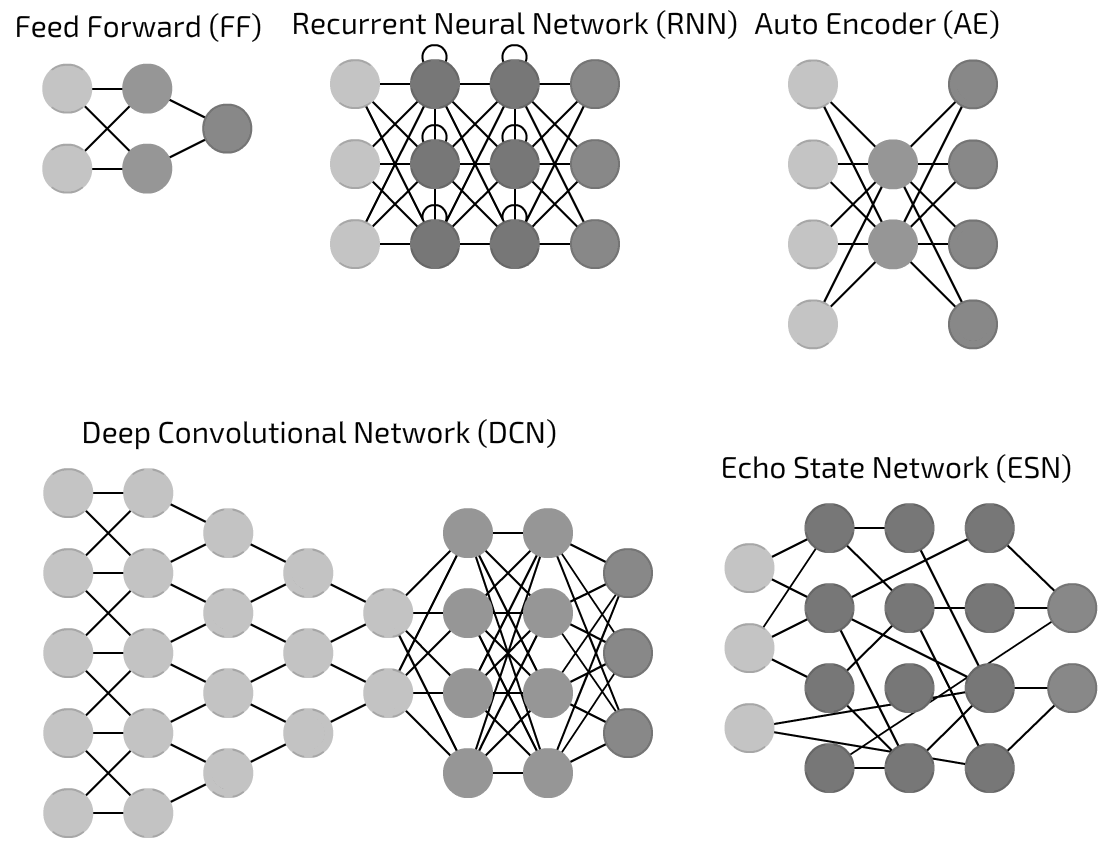
\includegraphics[width=0.95\textwidth]{img/tipologiereti.png}
		\caption{Esempi di reti neurali (credits: Andrew Tch, towardsdatascience.com)}
		\label{fig:tipologiereti}
	\end{center}
\end{figure}

\subsubsection{Backpropagation} La retropropagazione dell'errore, \textit{backward propagation of errors}$^{\cite{Rumelhart_1986}}$, è l'algoritmo più diffuso per l'addestramento supervisionato delle reti neurali. Questo algoritmo consiste di due fasi:
\begin{itemize}
    \item[-] \textit{Forward phase}, dove gli input vengono elaborati dalla rete neurale fino a produrre un output
    \item[-] \textit{Backward phase}, dove l'output prodotto è confrontato con la vera etichetta assegnata e, attraverso calcoli differenziali, vengono individuati i contributi all'errore di ogni nodo. Con questi contributi, attraverso un algoritmo di ottimizzazione (solitamente, la discesa di gradiente), vengono modificati i pesi delle connessione fra i nodi, partendo dai nodi output e risalendo la rete fino ai nodi input.
\end{itemize}
Questo algoritmo richiede quindi che le funzioni di attivazione dei nodi siano differenziabili, e può soffrire di un problema che prende il nome di \textit{vanishing/exploding gradient problem}$^{\cite{DBLP:journals/corr/abs-1211-5063}}$, o problema della scomparsa/esplosione del gradiente. Nel dettaglio, attraverso questo algoritmo ogni parametro del modello viene modificato, durante la \textit{backward phase}, in maniera proporzionale alla derivata parziale della funzione \textit{loss} rispetto al parametro stesso. Propagando all'indietro attraverso la regola della catena$^{(\ref{eq:catena})}$ dei gradienti compresi nell'intervallo $[0, 1]$, come nel caso di alcune funzioni di attivazione, il prodotto diventa tanto più piccolo quanto più è profonda la rete neurale o, viceversa, esplodere in caso di gradienti dai valori elevati.
\begin{equation}\label{eq:catena}
D\left[f(g(x))\right] = f'(g(x))\cdot g'(x)
\end{equation}
Questo problema viene mitigato dall'uso di funzioni di attivazioni diverse, come le già citate ReLU$^{(\ref{eq:fun_relu})}$ e softmax$^{(\ref{eq:fun_softmax})}$, o dall'uso di algoritmi di addestramento che fanno uso solo del segno del gradiente e non della sua norma, come l'algoritmo Rprop$^{\cite{Riedmiller92rprop-}}$.\\
Nelle reti neurali ricorrenti, un grande contributo alla mitigazione del problema è avvenuto grazie all'introduzione delle LSTM, \textit{Long Short-Term Memory}$^{\cite{10.1162/neco.1997.9.8.1735}}$, che mantengono informazioni sullo stato del modello senza propagarle attraverso funzioni non lineari.

\subsection{Continual Learning} L'addestramento di un modello di Machine Learning attraverso un \textit{training set} disponibile fin da subito e fornito interamente al modello è denominato "addestramento \textit{offline}", o \textit{offline training}. Esistono contesti, però, dove i dati necessari o utili all'addestramento non sono subito tutti disponibili, ma diventano tali col passare del tempo. Un esempio di questa situazione sono i sistemi di raccomandazione in servizi come Netflix o YouTube: essi imparano continuamente i gusti dell'utente, in modo da fornire suggerimenti su video e film sempre adatti ai gusti del momento. Questa situazione, in cui i dati di addestramento diventano disponibili col passare del tempo e cioè di addestramento continuativo, è detta "addestramento continuo", o \textit{continual learning}.\\
Nel caso dell'addestramento continuo, un grosso ostacolo è quello denominato \textit{catastrophic forgetting}$^{\cite{MCCLOSKEY1989109}}$: quando una rete neurale già addestrata viene addestrata su nuovi dati, essa tenderà a dimenticare ciò che ha appreso sui dati precedenti. Questa situazione è una manifestazione del cosiddetto dilemma della \textbf{plasticità-stabilità}: si ha stabilità quando la nuova conoscenza non interferisce con la vecchia conoscenza, mentre si parla di plasticità quando la nuova conoscenza migliora la conoscenza già appresa e viceversa. Questi due obiettivi sono in contrapposizione fra loro e mantenere un buon compromesso fra i due è uno degli obiettivi chiave degli algoritmi e attuale campo di studio.\\\\
In un mondo in continua e rapida evoluzione l'addestramento continuo diventa un approccio sempre più necessario, e apporta al Machine Learning un cambiamento di paradigma al pari dell'introduzione della filosofia Agile$^{\cite{agilemanifesto}}$ nel mondo dell'ingegneria del software: mentre in molti dei modelli di Machine Learning correnti l'addestramento è eseguito da zero e il modello viene utilizzato così com'è, con un procedimento comparabile ai primi approcci "a cascata" adottati nello sviluppo dei software, l'addestramento continuo fornisce a questo campo la possibilità di produrre modelli che vengono migliorati iterativamente ogni volta che è necessario senza dover addestrare un nuovo modello da zero. "Il parallelismo sta nell'equiparare i dati ai requisiti (arrivano in maniera continuativa e cambiano nel tempo) e l'addestramento alla fase di design e sviluppo che porta al prodotto software (che nel nostro caso è la funzione di predizione realizzata dal modello di Machine Learning)."$^{\cite{lomonaco_2019}}$
\section{Stato dell'Arte}
\subsection{Addestramento Continuo} L'ambito dell'addestramento continuo è in continua evoluzione. Negli ultimi anni, studi come \textit{Learning without Forgetting}$^{\cite{li2017learning}}$ o \textit{Overcoming catastrophic forgetting in neural networks}$^{\cite{kirkpatrick2017overcoming}}$ hanno affrontato il problema del \textit{catastrophic forgetting} proponendo soluzioni da adottare durante l'addestramento delle reti neurali. In \textit{Learning without Forgetting} viene proposto l'omonimo approccio, LWF, che non usa dati relativi alla conoscenza già appresa ma solo i nuovi dati relativi alla nuova conoscenza da apprendere, introducendo parametri del modello specifici per i nuovi dati ma che abbiano performance non impattanti sulla conoscenza già presente. Nel secondo studio viene proposto un algoritmo che prende il nome di \textit{Elastic Weight Consolidation}, o EWC, che interpreta i parametri da apprendere della rete neurale come spazi probabilistici, e rende meno probabile la modifica di quei parametri che risultano importanti per la conoscenza già appresa quando si addestra su nuova conoscenza.\\
Ulteriori studi hanno proposto approcci definiti \textit{reharsal} o di replay$^{\cite{DBLP:journals/corr/Lopez-PazR17},\cite{rolnick2019experience}}$. Queste tecniche consistono nel mantenere in memoria, all'interno di buffer, degli esempi della conoscenza passata selezionati secondo qualche politica. Durante le fasi di addestramento successive, ai nuovi dati vengono intervallati gli esempi mantenuti in memoria, così da consentire al modello di "ricordare" la conoscenza passata e mantenerla, mitigando così il \textit{catastrophic forgetting}.\\\\
Altri studi hanno proposto metriche per misurare le performance dell'apprendimento continuo e l'impatto che questo approccio ha sulla vecchia e nuova conoscenza, come in \textit{Gradient Episodic Memory for Continual Learning}$^{\cite{DBLP:journals/corr/Lopez-PazR17}}$ dove vengono proposte metriche per misurare il \textit{forward transfer}, FWT, e il \textit{backward transfer}, BWT: con queste due metriche si misura l'impatto che la nuova conoscenza ha sulla conoscenza, rispettivamente, già appresa e su quella che si andrà ad apprendere.\\\\
Altri recenti studi nell'ambito del continual learning si sono concentrati, ad esempio, sull'applicabilità pratica e l'ideazione di un'architettura in grado di manutenere modelli di Machine Learning in produzione e gestire la dinamicità e i cambiamenti sui dati$^{\cite{diethe2019continual}}$, oppure in ambiti come la \textit{human activity recognition} (HAR)$^{\cite{Jha_2021}}$, che riguarda il riconoscimento delle attività quotidiane delle persone attraverso dei sensori, o ancora l'acquisizione di informazioni dai social media per gestire al meglio situazioni di crisi$^{\cite{priyanshu2021continual}}$.\\
In tutti questi ambiti l'addestramento continuo si rivela fondamentale per adattare dinamicamente i modelli di Machine Learning al mutevole ambiente reale, senza la necessità di addestrare continuamente nuovi modelli da zero con l'ulteriore difficoltà costituita dal memorizzare dati anche molto vecchi portando a dataset di dimensioni elevate che aumentano il tempo necessario all'addestramento. Grazie all'addestramento continuo, invece, è possibile mantenere solo una parte degli esempi della conoscenza precedente, negli approcci cosiddetti di \textit{reharsal} o \textit{replay}, o non mantenerne affatto.\\\\
In molti studi, l'approccio all'addestramento continuo è stato suddiviso in tre scenari fondamentali$^{\cite{vandeven2019generative},\cite{vandeven2019scenarios}}$. Viene presa in considerazione una rete neurale che deve apprendere in maniera sequenziale una serie di task, dove con task si indica una qualsiasi attività che la rete neurale deve svolgere, ad esempio classificare le razze dei cani che appaiono in un immagine:
\begin{itemize}
    \item[-] \textbf{Task-IL}, o \textit{task incremental}: viene indicato il task a cui appartiene il problema, tra i task già appresi dal modello, e viene chiesto di risolverlo
    \item[-] \textbf{Domain-IL}, o \textit{domain incremental}: viene chiesto di risolvere il problema senza indicare il task a cui appartiene tra quelli appresi
    \item[-] \textbf{Class-IL}, o \textit{class incremental}: viene chiesto di risolvere il problema e anche di identificare a quale task esso appartiene.
\end{itemize}
Un dataset molto usato nell'ambito del Machine Learning è il MNIST, un database di cifre manoscritte che viene usato per valutare modelli, approcci e algoritmi riguardanti l'addestramento e il comportamento dei modelli di classificazione delle immagini (Figura \ref{fig:mnistexamples}).
\begin{figure}[h]
	\begin{center}
		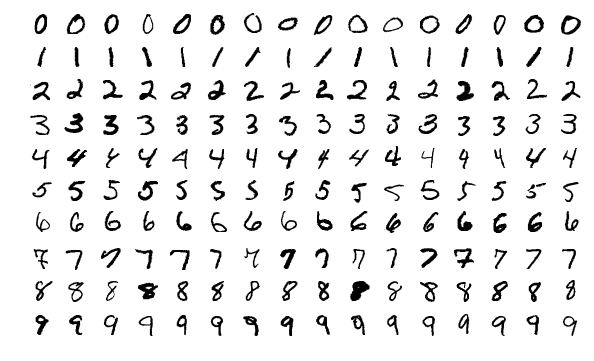
\includegraphics[width=0.75\textwidth]{img/MnistExamples.png}
		\caption{Esempio dei dati del MNIST (credits: Josef Steppan, Wikipedia)}
		\label{fig:mnistexamples}
	\end{center}
\end{figure}
Per meglio comprendere i tre scenari proposti, i task relativi al dataset MNIST possono essere individuati nei seguenti:
\begin{itemize}
    \item[-] Task 1: identificare tra 0 e 1
    \item[-] Task 2: identificare tra 2 e 3
    \item[-] Task 3: identificare tra 4 e 5
    \item[-] Task 4: identificare tra 6 e 7
    \item[-] Task 5: identificare tra 8 e 9
\end{itemize}
Con questi task, i tre scenari individuati diventano:
\begin{itemize}
    \item[-] \textbf{Task-IL}: dato il task, è la prima o la seconda classe? Ad esempio, identificare fra 0 e 1
    \item[-] \textbf{Domain-IL}: senza sapere il task, è la prima o la seconda classe? Ad esempio, identificare se è un numero pari (prima classe) o dispari (seconda classe)
    \item[-] \textbf{Class-IL}: senza sapere il task, che cifra è? Nell'esempio, individuare quale cifra è da 0 a 9
\end{itemize}
\subsection{Reti Neurali Ricorrenti}
Una rete neurale ricorrente, o RNN, è una rete neurale dove i neuroni, o alcuni di essi, sono collegati a sé stessi in un ciclo chiuso. Questo collegamento consente ai layer di una RNN di mantenere informazioni in maniera analoga ad uno stato interno, permettendo di modellare, ad esempio, i comportamenti dinamici di una sequenza temporale fornita come input, dove ogni dato dipende anche dai dati precedenti già ricevuti.\\
In letteratura esistono diverse architetture di reti neurali ricorrenti, ma molte di esse devono la loro esistenza a due nodi ricorrenti fondamentali: le \textit{Long Short-Term Memory}, LSTM$^{\cite{10.1162/neco.1997.9.8.1735}}$, e le \textit{Gated Recurrent Unit}, GRU$^{\cite{DBLP:journals/corr/ChoMGBSB14}}$ (Figura \ref{fig:rnnlstmgru}). 
\begin{figure}[h]
	\begin{center}
		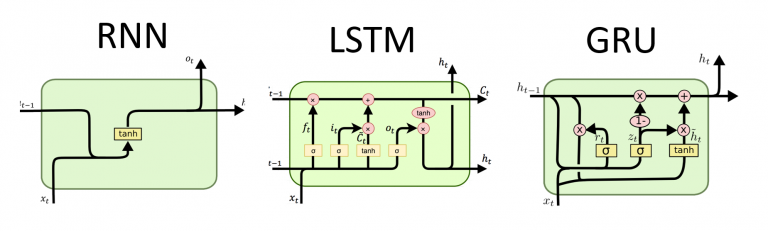
\includegraphics[width=0.95\textwidth]{img/rnnlstmgru.png}
		\caption{Schemi di nodi ricorrenti (credits: Michael Phi, towardsdatascience.com)}
		\label{fig:rnnlstmgru}
	\end{center}
\end{figure}
LSTM e GRU hanno meccanismi interni, chiamati \textit{gates} o cancelli, che regolano il flusso delle informazioni. Attraverso questi \textit{gate}, le unità apprendono quali dati sono importanti all'interno della sequenza e quali si possono ignorare, lasciando così al resto della rete solamente le informazioni che ritiene essere rilevanti per fare predizioni.\\\\
In una LSTM, i dati passano attraverso il \textit{forget gate}, che decide immediatamente quali informazioni è utile mantenere e quali ignorare. Dopodiché i dati passano attraverso l'\textit{input gate} assieme allo stato precedente dell'unità, che decide quali valori dello stato interno conviene aggiornare, e queste informazioni sono poi usate per aggiornare lo stato dell'unità. Infine, attraverso l'\textit{output gate} viene calcolato il nuovo stato interno dell'unità, che servirà all'input successivo.\\\\
Nelle GRU abbiamo un comportamento simile, ma la struttura dell'unità è semplificata. I dati passano subito attraverso il \textit{update gate}, che si comporta in modo simile ai \textit{gate} \textit{forget} e \textit{input} dell'LSTM, decidendo quali informazioni ignorare e quali mantenere. Dopodiché si attraversa il \textit{reset gate}, che decide cosa mantenere delle informazioni precedententemente analizzate. Avendo una struttura più semplificata, la GRU sono solitamente più veloci delle LSTM.
\subsection{Software e Hardware}
Negli ultimi anni sono nate diverse librerie software che consentono di realizzare modelli di Machine Learning performanti in breve tempo dei tipi più disparati, da semplici modelli lineari a reti neurali profonde convolutive e oltre.\\
Librerie open source come PyTorch, Tensorflow$^{\cite{abadi2016tensorflow}}$ e Keras, ma anche librerie proprietarie come Apple Core ML, IBM Watson e MATLAB Deep Learning Toolbox, hanno aperto le porte del Machine Learning a chiunque sia disposto a studiarle. Alcune librerie, come in particolare TensorFlow 2.0, possiedono API estremamente semplici che consentono di eseguire il preprocessing dei dataset, strutturare una rete neurale, addestrarla e valutarla con poche di righe di codice, e nonostante la semplicità essa consente comunque di mettere mano e andare a personalizzare ogni minimo aspetto di tutte le fasi, dal preprocessing al training. In letteratura sono disponibili anche moltissimi testi che consentono di approcciarsi facilmente al Machine Learning$^{\cite{chollet},\cite{geron}}$.\\\\
Anche a livello hardware gli ultimi anni hanno portato enormi sviluppi, grazie soprattutto all'industria videoludica e alle criptovalute che hanno spinto la ricerca e lo sviluppo di processori specializzati in calcolo parallelo e matriciale. Questi dispositivi, denominati \textit{Graphics Processing Unit} o GPU, consentono di ridurre esponenzialmente i tempi di addestramento delle reti neurali, abbassando ancora di più i requisiti per accedere a questo campo di studi e consentendo l'esecuzione di modelli di Machine Learning anche su un comune computer casalingo.\\
Inoltre, aziende come Google hanno sviluppato hardware realizzato ad hoc per le computazioni necessarie alle reti neurali, incrementando così ulteriormente la velocità e l'efficienza di questi modelli. Nel caso di Google, questo hardware è chiamato \textit{Tensor Processing Unit} o TPU.
\subsection{Applicazioni Future}
Alla luce degli attuali studi nell'ampio campo che è il Machine Learning, e in particolare riguardanti il continual learning e lo HSM, diventa chiaro come il futuro richiederà sempre più responsività ai sistemi predittivi e un sempre maggior grado di adattamento allo stato psico-fisico del momento dell'utente. Questa necessità di continua evoluzione ben si sposa con le caratteristiche del continual learning, e possibili applicazioni di questa sinergia continual learning -- HSM si possono individuare in diversi contesti, tra cui ad esempio:
\begin{itemize}
    \item[-] \textbf{Guida autonoma}.\\La crescente industria dei veicoli a guida autonoma ha portato ad uno sviluppo in moltissimi campi del Machine Learning$^{\cite{huang2020autonomous}}$, in particolare nel campo dell'\textit{object recognition}$^{\cite{Carranza_Garc_a_2021}}$, del \textit{behavioral planning}$^{\cite{6856582}}$ e altri ancora. L'\textit{autonomous driving} negli ultimi anni è, senza dubbio, uno dei motori principali nello sviluppo della disciplina del Machine Learning.\\
    Un veicolo a guida autonoma che sappia adattarsi allo stato psico-fisico attuale del conducente può portare a grossi benefici: ad esempio, essere in grado di modificare il proprio andamento per accomodare uno stato di malessere mitigando così il rischio di incidenti, o poter proporre tappe durante il percorso a seconda della condizione dei passeggeri portando così a più piacevole utilizzo del sistema da parte degli utenti.
    \item[-] \textbf{Intrattenimento}.\\L'industria dell'intrattenimento si è sempre interessata alle nuove tecnologie, puntando alla novità del momento in modo da raggiungere un pubblico sempre più ampio: ad esempio, la tecnologia degli schermi 3D o della realtà virtuale.\\
    Un sistema adattivo di riconoscimento dello stato psico-fisico dello spettatore o del videogiocatore può portare a esperienze multimediali più realistici e responsivi, che ad esempio possano adattare la propria narrazione o l'atmosfera proposta all'utente in maniera da sfruttare, o alleviare, eventuali emozioni che nascono nello spettatore.
    %\item[-] TODO altri esempi: interfacce che si modulano in base allo stato mentale del momento?
\end{itemize}
In tutti questi ambiti, per poter ottenere ottimi risultati, i sistemi devono essere in grado di adattarsi e specializzarsi nel riconoscere lo stato psico-fisico del singolo utente (ad esempio, il conducente proprietario del veicolo o il videogiocatore che possiede la console) ottenendo così sistemi calibrati e personalizzati in base alle caratteristiche e alle esigenze del singolo utente.\\\\
Questa sinergia risulta ancora poco studiata in letteratura, quindi può essere utile mettere sotto esame alcune tecniche di addestramento continuo attualmente studiate per giudicare la loro applicabilità o meno in contesti di \textit{human state monitoring}, così da concludere se siano necessari ulteriori sforzi in questa direzione per poter realizzare, in futuro, sistemi sempre più integrati con l'uomo e interfacce uomo-macchina sempre più intuitive e adattive. Valutare fin da subito l'applicabilità di questa sinergia è fondamentale in un campo di studi che si muove così in fretta come quello del Machine Learning.

  % obiettivi della ricerca e degli esperimenti
    \chapter{Dataset}
Ai fini del progetto, il primo elemento necessario per poter valutare correttamente la sinergia continual learning -- Human State Monitoring sono dei dati raccolti riguardanti quest'ultimo. I dati dovrebbero provenire da più soggetti, per correttezza statistica, e riguardare diversi aspetti biometrici della persona: battito cardiaco, sudorazione, respirazione\ldots\\\\
I dataset selezionati ai fini di questa comparazione sono due, che seguono.
\section{WESAD}
Il dataset WESAD$^{\cite{10.1145/3242969.3242985}}$, acronimo di \textit{WEarable Stress and Affect Detection}, contiene dati raccolti da 15 soggetti durante uno studio effettuato in laboratorio riguardante i livelli di stress misurati tramite sensori biometrici e di movimento indossabili. Il dataset classifica questi dati in tre scale: neutralità, stress e divertimento.\\
I dispositivi usati per la raccolta dei dati sono due: uno indossato sul petto (RespiBAN) e uno indossato sul polso (Empatica E4).\\\\Il RespiBAN, indossato sul petto, raccoglie dati campionati a 700 Hz su:
\begin{itemize}
    \item[-] Elettrocardiogramma (ECG)
    \item[-] Attività elettrodermica (EDA)
    \item[-] Elettromiogramma (EMG)
    \item[-] Respirazione
    \item[-] Temperatura corporea
    \item[-] Accelerazione sui tre assi
\end{itemize}
L'Empatica E4, indossato sul polso, monitora con frequenza di campionamento eterogenea:
\begin{itemize}
    \item[-] Pulsazioni (BVP), a 64Hz
    \item[-] Attività elettrodermica (EDA), a 4 Hz
    \item[-] Temperatura corporea, a 4 Hz
    \item[-] Accelerazione sui tre assi, a 32 Hz
\end{itemize}
La quantità di dati contenuti in questo dataset lo rende un ottimo strumento nell'addestramento di modelli di machine learning riguardanti l'ambiente dello HSM. Dati come le pulsazioni, la temperatura e l'elettrocardiogramma sono precisissimi indicatori biometrici dello stato psico-fisico di una persona e pertanto sono estremamente utili alle reti neurali per dedurre lo stato psico-fisico di soggetto.
\subsection{Preprocessing}
Una volta caricato il dataset, i dati sono stati concatenati e ricampionati a 32 Hz, attraverso la libreria \texttt{SciPy}.
\lstinputlisting[style=myPython, firstnumber=31, firstline=31, lastline=42]{code/wesad_data.py}
Dopodiché, l'insieme delle features è stato standardizzato ponendo media pari a 0 e deviazione standard uguale a 1
\lstinputlisting[style=myPython, firstnumber=46, firstline=46, lastline=46]{code/wesad_data.py}
Sono state ricampionate le etichette e sono state rimosse l'etichetta 0, corrispondente ad una condizione di neutralità, e le etichette 5, 6 e 7 poichè secondo le indicazioni del dataset sono corrispondenti a dati da ignorare.
\lstinputlisting[style=myPython, firstnumber=50, firstline=50, lastline=52]{code/wesad_data.py}
\lstinputlisting[style=myPython, firstnumber=56, firstline=56, lastline=57]{code/wesad_data.py}
\lstinputlisting[style=myPython, firstnumber=86, firstline=86, lastline=87]{code/wesad_data.py}
I dati sono poi raccolti in sottosequenze di 100 punti relativi alla stessa etichetta, corrispondenti a circa 3 secondi, e per ogni etichetta vengono estratte 100 di queste sottosequenze.
\lstinputlisting[style=myPython, firstnumber=62, firstline=62, lastline=82]{code/wesad_data.py}
Dai dati viene poi estratto un test set. Questo ci lascia con un test set di 1500 elementi e un training set da 4500 elementi suddivisi come specificato nella tabella \ref{tab:splittedwesad}.

\section{ASCERTAIN }
ASCERTAIN$^{\cite{10.1145/2818346.2820736}}$, acronimo di \textit{multimodal databASe for impliCit pERsonaliTy and Affect recognitIoN}, è un dataset contenente dati provenienti da 58 soggetti raccolti con sensori fisiologici commerciali e classifica le informazioni su diverse scale: incitamento, valenza, investimento, apprezzamento e familiarità. Il dataset contiene anche dati relativi all'attività facciale dei soggetti registrati con sensori comuni, oltre ai dati sull'elettroencefalogramma (EEG), elettrocardiogramma (ECG) e sulle risposte galvaniche della pelle (GSR).\\\\
Il motivo principale per cui è stato selezionato ASCERTAIN sono i dati sui movimenti facciali dei soggetti. In contesti reali, dove non sempre è possibile raccogliere dati sull'utente mediante sensori biometrici applicati sul corpo del soggetto, spesso è disponibile solamente una o più videocamere che lo riprendono. Poter sfruttare questi dati non invasivi per poter trarre conclusioni relative allo HSM può rivelarsi quindi molto utile in applicazioni reali.
\subsection{Preprocessing}
Dal dataset sono stati esclusi due soggetti poiché i loro dati risultavano imprecisi o incompleti. Ogni soggetto rimanente è stato caricato e per ognuno sono state create le etichette seguendo la seguente suddivisione basata sui valori di incitamento e valenza specificati, che corrispondono ai quadranti del grafico cartesiano creato dai due valori:
\begin{itemize}
    \item[-] Label 0, corrispondente a valori di incitamento $> 3$ e valenza $> 0$
    \item[-] Label 1, corrispondente a valori di incitamento $> 3$ e valenza $\leq 0$
    \item[-] Label 2, corrispondente a valori di incitamento $\leq 3$ e valenza $> 0$
    \item[-] Label 3, corrispondente a valori di incitamento $\leq 3$ e valenza $\leq 0$
\end{itemize}
\lstinputlisting[style=myPython, firstnumber=40, firstline=40, lastline=51]{code/ascertain_data2.py}
I dati sono poi ripuliti dai valori mancanti, ricampionati a 32 Hz e concatenati fra loro.
\lstinputlisting[style=myPython, firstnumber=55, firstline=55, lastline=58]{code/ascertain_data2.py}
\lstinputlisting[style=myPython, firstnumber=62, firstline=62, lastline=64]{code/ascertain_data2.py}
\lstinputlisting[style=myPython, firstnumber=68, firstline=68, lastline=76]{code/ascertain_data2.py}
Vengono poi costruite le sottosequenze, da 160 elementi ciascuna (5 secondi), mantenendo un bilanciamento fra le diverse classi.
\lstinputlisting[style=myPython, firstnumber=80, firstline=80, lastline=80]{code/ascertain_data2.py}
\lstinputlisting[style=myPython, firstnumber=82, firstline=82, lastline=104]{code/ascertain_data2.py}
Come per WESAD, anche da ASCERTAIN viene estratto un test set, il che ci lascia con un test set da 720 elementi e un training set da 2160 elementi suddivisi come indicato nella tabella \ref{tab:splittedascertain}

\begin{table}[h]
    \parbox{.45\linewidth}{
    	\begin{center}
    		\begin{tabular}{l|c}
    		     \textbf{Soggetto} & \textbf{Dati}\\
    		     \hline
    		     S2 & 287 \\
    		     S3 & 287 \\
    		     S4 & 298 \\
    		     S5 & 298 \\
    		     S6 & 297 \\
    		     S7 & 303 \\
    		     S8 & 309 \\
    		     S9 & 292 \\
    		     S10 & 313 \\
    		     S11 & 292 \\
    		     S13 & 308 \\
    		     S14 & 297 \\
    		     S15 & 305 \\
    		     S16 & 313 \\
    		     S17 & 301 \\
    		     \hline
    		     Totale & 4500
    		\end{tabular}
    		\caption{Datataset WESAD}
    		\label{tab:splittedwesad}
    	\end{center}
	}
    \parbox{.45\linewidth}{
    	\begin{center}
    		\begin{tabular}{l|c}
    		     \textbf{Soggetto} & \textbf{Dati}\\
    		     \hline
    		     S0 & 95 \\
    		     S1 & 75 \\
    		     S2 & 148 \\
    		     S3 & 154 \\
    		     S4 & 153 \\
    		     S5 & 208 \\
    		     S6 & 131 \\
    		     S7 & 115 \\
    		     S8 & 119 \\
    		     S9 & 206 \\
    		     S10 & 119 \\
    		     S11 & 78 \\
    		     S12 & 74 \\
    		     S13 & 109 \\
    		     S14 & 72 \\
    		     S15 & 84 \\
    		     S16 & 220 \\
    		     \hline
    		     Totale & 2160
    		\end{tabular}
    		\caption{Datataset ASCERTAIN}
    		\label{tab:splittedascertain}
    	\end{center}
    }
\end{table}
\section{Differenze fra i due dataset}
Uno degli elementi da considerare quando si addestra una rete neurale è il bilanciamento dei dati presi in considerazione per l'addestramento.\\
Andando ad analizzare nel dettaglio la struttura dei due dataset considerati, diventa evidente la decisa sovrarappresentanza della classe 0 nel dataset ASCERTAIN, mentre le classi nel dataset WESAD risultano molto più bilanciate. Questo è anche dovuto all'aver scelto delle classi fittizie, per quanto riguarda ASCERTAIN, che ha evidenziato come non tutti i soggetti abbiano prodotto dati bilanciati rispetto alle nuove classi selezionate. Anche eseguendo un bilanciamento successivo, ovvero eliminando gli esempi in eccesso sulla prima classe, si raggiungono misurazioni analoghe a quelle presentate.

Bilanciando il dataset ASCERTAIN attraverso la produzione di soggetti fittizi, ognuno contenente dati presi da tutti i soggetti in maniera bilanciata rispetto alle nuove classi, otteniamo immediatamente risultati sensibilmente migliori, con accuratezze a volte anche doppie rispetto allo stesso metodologia sul dataset ASCERTAIN originale. Questo rende evidente l'importanza dell'avere dati di addestramento bilanciati, quindi esempi in quantità simile per ognuna delle etichette possibili.
\begin{figure}[h]
    \begin{minipage}[b]{0.5\textwidth}
		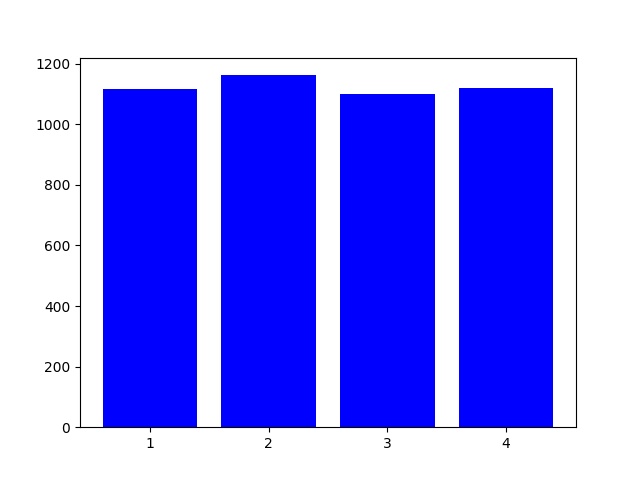
\includegraphics[width=\textwidth]{img/graphs/wesad_dataset.png}
		\caption{Presenza delle classi su dataset WESAD}
		\label{fig:wesadclasses}
	\end{minipage}
    \hfill
    \begin{minipage}[b]{0.5\textwidth}
		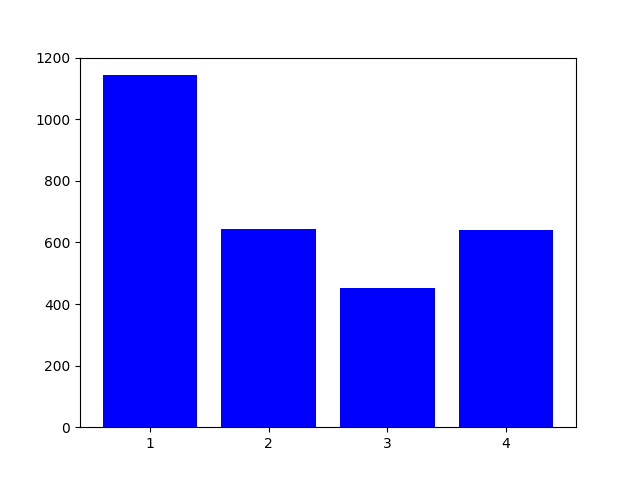
\includegraphics[width=\textwidth]{img/graphs/ascertain_dataset.png}
		\caption{Presenza delle classi su dataset ASCERTAIN}
		\label{fig:ascertainclasses}
	\end{minipage}
\end{figure}
% aggiungere queste parti? \/
% presi in considerazione diversi (WESAD, HHAR (\cite{10.1145/2809695.2809718}) per attività fisiche, PAMAP2 (\cite{6246152}) per dati cuore e movimento, OPPORTUNITY (\cite{5573462}) per movimenti del corpo, ASCERTAIN)
% WESAD e ASCERTAIN scelti principalmente per i dati biometrici contenuti, ASCERTAIN (\cite{10.1145/2818346.2820736}) in particolare dati facciali utili in contesti reali dove non è sempre possibile attaccare sensori all'utente, mentre WESAD concentrato principalmente sullo stress quindi utile in altri contesti  % dataset scelti e preprocessing eseguito
    \chapter{Metodologie}
In questo capitolo verranno delineate nel dettaglio le varie metodologie scelte per la realizzazione della comparazione fra alcune strategie di addestramento continuo triviali applicate ai dataset di Human State Monitoring presentati nel precedente capitolo.

\section{Metriche}
Per poter confrontare fra loro le diverse strategie, fin da subito è apparsa chiara la necessità di metriche che misurassero con precisione alcune caratteristiche fondamentali delle metodologie di addestramento continuo, in particolare: l'accuratezza sul test set, l'accuratezza media sulle classi e i \textit{forward} e \textit{backward transfer} per poter misurare l'impatto della nuova conoscenza sulla conoscenza precedentemente appresa e su quella ancora da acquisire.
\subsection{Accuratezza}
Con "accuratezza" si intende la misura della percentuale di previsioni corrette che il modello di machine learning ottiene su un test set, cioè un insieme di dati a cui il modello non è stato esposto durante le sessioni di addestramento.\\
Per poter misurare l'accuratezza su un insieme di dati, l'API di TensorFlow mette a disposizione un comando che valuta un modello di machine learning applicato ai dati passati come parametro:
\begin{lstlisting}[style = myPython]
model.evaluate(Xtest, ytest)
\end{lstlisting}
Questa chiamata ritorna il valore assunto dalla funzione di loss al termine della valutazione e le metriche che vengono specificate durante la compilazione del modello. Compilando il modello con il seguente comando
\begin{lstlisting}[style = myPython]
model.compile(loss = 'categorical_crossentropy', optimizer = opt, metrics = ['accuracy'])
\end{lstlisting}
otterremo un modello la cui funzione di loss è la cross-entropia categorica, usata per modelli che devono classificare dati appartenenti ad una sola classe fra diverse disponibili, e come metrica aggiuntiva richiediamo l'accuratezza. Così facendo, con
\begin{lstlisting}[style = myPython]
model.evaluate(Xtest, ytest)[1]
\end{lstlisting}
otteniamo la misura dell'accuratezza che il modello \texttt{model} ottiene sul test set composto dai dati \texttt{Xtest} e dalle etichette \texttt{ytest}.\\\\
La misura di accuratezza indicata nei risultati è l'accuratezza media ottenuta dal modello durante le varie sessioni di addestramento.
\subsection{ACC, FWT e BWT}
Queste tre metriche sono state tratte e adattate dalla pubblicazione \textit{Gradient Episodic Memory for Continual Learning}$^{\cite{DBLP:journals/corr/Lopez-PazR17}}$, e si basano sulla costruzione di una matrice $R \in \mathbb{R}^{E\times T}$. Con $T$ si indica il numero di classi del problema in esame, e ogni volta che il modello finisce una sessione di addestramento tra le $E$ che vengono eseguite si va a valutare la sua \textit{test performance} su tutte le $T$ classi. Così facendo, si calcolano le $R_{i,j}\in R$ valutazioni dell'accuratezza del test di classificazione del modello sulla classe $t_j$ dopo aver osservato gli esempi della $i$-esima sessione di addestramento. Inoltre, una volta creato il modello con una inizializzazione dei pesi casuale si calcola $\overline{b}$, valutazione delle accuratezza nei test sui vari task.\\
Possiamo ora definire le tre metriche:
\begin{itemize}
    \item[-] \textbf{ACC}, \textit{Accuracy} o accuratezza
        \begin{equation}\label{eq:fun_acc}
            ACC = \frac{1}{T}\cdot\sum_{i=1}^T R_{E,i}
        \end{equation}
    Va a misurare l'accuratezza del modello su tutti le $T$ classi a fine addestramento
    \item[-] \textbf{BWT}, \textit{Backward Transfer} o trasferimento all'indietro
        \begin{equation}\label{eq:fun_bwt}
            BWT = \frac{1}{T-1}\cdot\sum_{i=1}^T\left(\frac{1}{E}\sum_{j=1}^E R_{E,i} - R_{j,i}\right)
        \end{equation}
    Valuta l'influenza che ha una sessione di apprendimento sulle precedenti, valutando l'impatto che ha avuto sulle valutazioni dell'accuratezza in fase di test. Si ha un BWT positivo quando una sessione di addestramento migliora l'accuratezza delle precedenti già valutate, mentre un valore negativo indica che la sessione di addestramento ha deteriorato l'accuratezza che si otteneva grazie alla precedente conoscenza. Non è significativo parlare di BWT durante la prima sessione di addestramento.\\
    Un BWT fortemente negativo evidenzia il verificarsi del fenomeno del \textit{catastrophic forgetting}.
    \item[-] \textbf{FWT}, \textit{Forward Transfer} o trasferimento in avanti
        \begin{equation}\label{eq:fun_fwt}
            FWT = \frac{1}{T-1}\cdot\sum_{i=1}^T\left(\frac{1}{E}\sum_{j=1}^E R_{j,i} - \overline{b}_i\right)
        \end{equation}
    Serve per misurare l'influenza che la sessione di apprendimento ha sulla conoscenza ancora da apprendere. In particolare, un FWT positivo è possibile quando il modello è in grado di realizzare lo \textit{zero-shot} learning, cioè di apprendere informazioni sui task futuri senza essere esposto ad esempi da apprendere, per esempio sfruttando la struttura interna della conoscenza in caso di task simili.\\
    Non è significativo parlare di FWT durante l'ultima sessione di addestramento.
\end{itemize}
Tra queste tre, quella senza dubbio più interessante ai fini dell'esperimento è il BWT. Diventa particolarmente importante evitare gli scenari che portano al \textit{catastrophic forgetting}: nel nostro caso, uno scenario simile porterebbe a dimenticare esempi di HSM passati e a far sì che il modello si basi solamente sull'esperienza recente, rischiando di dimenticare importanti esempi passati di stati d'animo e di conseguenza a non saper più riconoscerli correttamente.\\\\
Più grandi sono queste metriche, migliore è il comportamento del modello in esame. A parità di ACC, si preferisce il modello con maggior BWT e FWT che denoterebbe un miglior trasferimento della conoscenza attraverso i task e le sessioni di training.
\subsection{Altre metriche}
Le altre metriche raccolte durante gli esperimenti sono le seguenti:
\begin{itemize}
    \item[-] \textbf{Numero di epoche} medio, e deviazione standard\\
    Questa misurazione fornisce una indicazione sul tempo di convergenza delle reti neurali selezionate sui dati, così da poter stimare le loro prestazioni su hardware diversi da quello di test.
    \item[-] \textbf{Tempo di addestramento} medio, e deviazione standard\\
    Gli esperimenti sono eseguiti su un personal computer comune, sfruttando le ottimizzazioni messe a disposizione dall'utilizzo di una GPU per i calcoli. Nello specifico, le computazioni sono state eseguite su una macchina che montava una GPU nVidia GeForce GTX 1070 con 6 Gb di memoria dedicata, una CPU Intel i5 3570 e 12 Gb di RAM.\\% CUDA 10.1 https://ai-benchmark.com/ranking_deeplearning.html
    Il tempo di addestramento è calcolato come la media dei tempi impiegati delle varie sessioni di addestramento.
    \item[-] \textbf{Quantità di memoria} media\\
    Metrica utile per valutare l'impatto sulla memoria del sistema che andrà poi a utilizzare il modello addestrato. Un elevato consumo di memoria può portare alla esclusione di dispositivi portatili o con specifiche particolari.
\end{itemize}

\section{Baseline: l'addestramento offline}
L'approccio classico all'addestramento di un modello di machine learning avviene raccogliendo i dati di addestramento e sottoponendoli al modello in una singola sessione di addestramento. Questa metodologia è statica e produce un modello che sui futuri dati si comporterà tanto meglio quanto essi saranno simili ai dati di addestramento.\\
La scelta di usare questa metodologia classica come baseline è stata guidata dal principio che, avendo tutti i dati a disposizione in una sola volta, la rete neurale risultante dovrebbe ottenere le migliori prestazioni possibili sul test set una volta che questo viene sottoposto, e quindi fornisce un "limite superiore" all'accuratezza delle metodologie continue. Una strategia di addestramento continuo è tanto migliore quanto più si avvicina alle performance che la stessa rete neurale otterrebbe se venisse addestrata su tutti i dati in maniera offline o, se possibile, quando la supera.\\\\
L'addestramento offline è quindi realizzato seguendo il seguente pseudo-algoritmo, applicabile sia a WESAD che ad ASCERTAIN:
\begin{enumerate}
    \item \textbf{Creare e compilare la rete neurale} che verrà poi addestrata.\\
    La creazione della rete neurale, attraverso la API Sequential di TensorFlow, è analoga per entrambi i dataset a meno della struttura interna. L'esempio seguente è tratto dall'addestramento offline per WESAD, e costruisce una rete neurale con due layer da 18 unità GRU e un layer output da 4 unità, corrispondenti alle 4 classi del dataset.
    \lstinputlisting[style=myPython, firstnumber=22, firstline=22, lastline=30]{code/wesad_totaltrain.py}
    \item \textbf{Caricare il dataset}, composto da training set e test set.\\
    Come precedentemente spiegato, i dataset sono divisi in training set e test set, e il training set è ulteriormente diviso fra i soggetti dei due studi. In entrambi i casi quindi, per quanto riguarda la metodologia offline, viene caricato il test set così come viene fornito, mentre il training set è realizzato concantenando fra loro i dati di tutti i soggetti. Esempio, sempre tratto da WESAD:
    \lstinputlisting[style=myPython, firstnumber=35, firstline=35, lastline=47]{code/wesad_totaltrain.py}
    \lstinputlisting[style=myPython, firstnumber=51, firstline=51, lastline=52]{code/wesad_totaltrain.py}
    Il training set è ulteriormente diviso in training set e validation set, utilizzato per monitorare l'andamento dell'addestramento e implementare la fermata anticipata dell'addestramento:
    \lstinputlisting[style=myPython, firstnumber=56, firstline=56, lastline=56]{code/wesad_totaltrain.py}
    \item \textbf{Addestramento} e risultati.\\
    Una volta preparato il dataset, si può dare il via all'addestramento. Prima di esso si preparano, sempre grazie all'API di TensorFlow, le due callback usate durante gli esperimenti: la creazione di grafici attraverso TensorBoard e la fermata anticipata in base all'andamento del valore della funzione di loss sul validation set:
    \lstinputlisting[style=myPython, firstnumber=59, firstline=59, lastline=68]{code/wesad_totaltrain.py}
    I risultati sono poi proiettati in output sul terminale:
    \lstinputlisting[style=myPython, firstnumber=70, firstline=70, lastline=73]{code/wesad_totaltrain.py}
\end{enumerate}
La metodologia offline, come visto, è immediata e grazie alle API di TensorFlow anche semplice da implementare. Essa è stata utilizzata anche per poter selezionare la rete neurale usata per il dataset relativo, una per WESAD e una per ASCERTAIN e che è poi stata usata su ciascun esperimento, in base all'accuratezza finale raggiunta.

\section{Metodologie di Addestramento Continuo}
Al centro di questo progetto ci sono le metodologie di addestramento continuo. Ne sono state selezionate alcune: 3 tecniche di replay e 2 tecniche che non sfruttano esempi già visti.\\\\
Per realizzare il flusso di dati necessario a implementare una strategia di addestramento continuo, le quali richiedono che i dati di addestramento non siano subito tutti disponibili ma che lo diventino nel tempo, i soggetti di entrambi i dataset sono stati mantenuti divisi per soggetto e raggruppati a coppie, per poi essere sottoposti all'addestramento della rete neurale una coppia per volta. Le tabelle \ref{tab:coppiewesad} e \ref{tab:coppieascertain} mostrano la suddivisione a coppie rispettivamente per il dataset WESAD e il dataset ASCERTAIN.
\begin{table}[h]
    \parbox{.45\linewidth}{
    	\begin{center}
    		\begin{tabular}{l|c}
    		     \textbf{Sessione} & \textbf{Coppie}\\
    		     \hline
    		     1 & S2, S3 \\
    		     2 & S4, S5 \\
    		     3 & S6, S7 \\
    		     4 & S8, S9 \\
    		     5 & S10, S11 \\
    		     6 & S13, S14 \\
    		     7 & S15, S16 \\
    		     \multicolumn{1}{c}{}
    		\end{tabular}
    		\caption{Suddivisione a coppie del dataset WESAD}
    		\label{tab:coppiewesad}
    	\end{center}
	}
    \parbox{.45\linewidth}{
    	\begin{center}
    		\begin{tabular}{l|c}
    		     \textbf{Sessione} & \textbf{Coppie}\\
    		     \hline
    		     1 & S0, S1 \\
    		     2 & S2, S3 \\
    		     3 & S4, S5 \\
    		     4 & S6, S7 \\
    		     5 & S8, S9 \\
    		     6 & S10, S11 \\
    		     7 & S12, S13 \\
    		     8 & S14, S15 \\
    		\end{tabular}
    		\caption{Suddivisione a coppie del dataset ASCERTAIN}
    		\label{tab:coppieascertain}
    	\end{center}
    }
\end{table}\\
Per poter misurare le metriche ACC, BWT e FWT delle metodologie di continual learning, in ogni esperimento viene prima preparato il test set suddividendolo nelle varie classi:
\lstinputlisting[style=myPython, firstnumber=21, firstline=21, lastline=22]{code/wesad_continualtrain.py}
\lstinputlisting[style=myPython, firstnumber=24, firstline=24, lastline=44]{code/wesad_continualtrain.py}
Subito dopo, appena viene creato il modello, vengono inizializzate le variabili necessarie e il vettore $\overline{b}$:
\lstinputlisting[style=myPython, firstnumber=57, firstline=57, lastline=64]{code/wesad_continualtrain.py}
Al termine di ogni sessione di addestramento, cioè appena concluso l'addestramento su una coppia, vengono calcolati gli $R_{i,j}$:
\lstinputlisting[style=myPython, firstnumber=97, firstline=97, lastline=97]{code/wesad_continualtrain.py}
Infine, al termine dell'ultima sessione di addestramento, vengono calcolate le varie metriche:
\lstinputlisting[style=myPython, firstnumber=99, firstline=99, lastline=118]{code/wesad_continualtrain.py}

\subsection{Naive}
La prima metodologia continua sperimentata è chiamata \textit{naive}. Questa metodologia consiste nel fornire al modello una coppia alla volta come training set, senza ulteriori elaborazioni: la semplicità di questa metodologia la rende molto facile da implementare, ma anche esposta alle problematiche intrinseche dell'apprendimento continuo esposte precedentemente. Questa metodologia è stata descritta in alcuni studi pioneristici nel campio dell'apprendimento continuo, come \cite{Ring2004CHILDAF}.\\\\
Nel dettaglio, inizialmente vengono stabilite le coppie:
\lstinputlisting[style=myPython, firstnumber=66, firstline=66, lastline=66]{code/wesad_continualtrain.py}
Ogni coppia è caricata e concatenata, per formare il training set della sessione che viene poi diviso in training set e validation set:
\lstinputlisting[style=myPython, firstnumber=68, firstline=68, lastline=71]{code/wesad_continualtrain.py}
\lstinputlisting[style=myPython, firstnumber=73, firstline=73, lastline=74]{code/wesad_continualtrain.py}
\lstinputlisting[style=myPython, firstnumber=83, firstline=83, lastline=83]{code/wesad_continualtrain.py}
Infine il modello è addestrato sul training set e validato sul validation set appena prodotti, sono calcolate le metriche ed esposte in output.
\subsection{Replay}  % una percentuale, di solito 25%
Questa è la prima tecnica di replay provata, ed anche la più semplice. Questa metodologia consiste nel mantenere una percentuale del training set utilizzato per addestrare la rete neurale durante l'attuale sessione di addestramento e usarla insieme al training set, cioè alla coppia di soggetti, della sessione di addestramento successiva. Anche questa metodologia è di facile implementazione e la sua filosofia è trattata in studi come \cite{rolnick2019experience}.\\\\
Subito prima di avviare l'addestramento, vengono inizializzate le due variabili che conterranno il training set:
\lstinputlisting[style=myPython, firstnumber=65, firstline=65, lastline=65]{code/wesad_continualreplaytrain.py}
Appena caricati i soggetti, viene costruito il training set mantenendo ciò che è stato trattenuto dalla sessione precedente e memorizzato in \texttt{X}, se presente:
\lstinputlisting[style=myPython, firstnumber=74, firstline=74, lastline=79]{code/wesad_continualreplaytrain.py}
A fine sessione di addestramento, si trattiene la percentuale di replay (nell'esempio, il 25\%):
\lstinputlisting[style=myPython, firstnumber=100, firstline=100, lastline=100]{code/wesad_continualreplaytrain.py}

\subsection{Cumulative}  % si mantengono gli esempi precedenti nei successivi addestramenti, così all'arrivo dell'ultima coppia di soggetti il training set è uguale al caso offline
Con questa metodologia, si intende mantenere di volta in volta l'intero training set accumulando le coppie di soggetti che diventano disponibili. Così facendo, all'arrivo dell'ultima coppia di soggetti si avrà un training set pari al training set usato nella metodologia offline, contenendo tutti i dati di tutti i precedenti soggetti, con la differenza che si addestra una rete neurale che è stata già addestrata su tutte le coppie presenti nel training set ad eccezione dell'ultima arrivata. Questa metodologia può essere considerata una versione particolare della metodologia di replay precedente: abbiamo un replay del 100\% dei dati, così che tra una sessione di addestramento e l'altra si mantiene l'intero training set utilizzato.\\\\
Viene realizzato nel seguente modo: la prima sessione di addestramento è realizzata sulla prima coppia di soggetti partendo dalla rete neurale inizializzata con i pesi casuali, mentre mano a mano che arrivano le coppie successive esse vengono concatenate al training set della sessione precedente e la rete è addestrata senza reinizializzare i pesi, cioè mantenendo l'addestramento precedente. Una problematica da tenere in considerazione è la memoria necessaria richiesta per mantenere i training set nella loro totalità: durante l'ultima sessione di addestramento avremo un training set corrispondente al training set usato nella metodologia offline, di conseguenza mantenere in memoria tutti i dati necessari potrebbe non essere praticabile in contesti reali.
\subsection{Episodic}  % si mantengono di volta in volta m esempi per ogni classe tratti dal training set
Nelle precedenti tecniche di replay si mantenevano tutti i dati o un sottoinsieme scelto casualmente del training set. Con questa tecnica, invece, viene mantenuto di sessione in sessione un numero fisso $m$ di esempi per ogni etichetta, così da avere un replay bilanciato rispetto alle classi. L'idea dietro questa tecnica di replay è descritta nello studio "Gradient Episodic Memory for Continuum Learning"$^{\cite{DBLP:journals/corr/Lopez-PazR17}}$.\\\\
Subito prima di avviare l'addestramento, vengono inizializzate le "memorie episodiche" e il parametro $m$, che indica quanti esempi per classe mantenere (nell'esempio, $m = 70$):
\lstinputlisting[style=myPython, firstnumber=68, firstline=68, lastline=69]{code/wesad_episodic.py}
Al termine di una sessione di addestramento, il training set appena usato è suddiviso per classi:
\lstinputlisting[style=myPython, firstnumber=105, firstline=105, lastline=108]{code/wesad_episodic.py}
\lstinputlisting[style=myPython, firstnumber=112, firstline=112, lastline=115]{code/wesad_episodic.py}
\lstinputlisting[style=myPython, firstnumber=119, firstline=119, lastline=122]{code/wesad_episodic.py}
\lstinputlisting[style=myPython, firstnumber=126, firstline=126, lastline=129]{code/wesad_episodic.py}
Ogni sottoinsieme è mescolato, per evitare di mantenere sempre i soliti esempi, e da ognuno ne vengono presi $m$:
\lstinputlisting[style=myPython, firstnumber=109, firstline=109, lastline=111]{code/wesad_episodic.py}
\lstinputlisting[style=myPython, firstnumber=116, firstline=116, lastline=118]{code/wesad_episodic.py}
\lstinputlisting[style=myPython, firstnumber=123, firstline=123, lastline=125]{code/wesad_episodic.py}
\lstinputlisting[style=myPython, firstnumber=130, firstline=130, lastline=132]{code/wesad_episodic.py}
Infine, viene formato il training set che andrà a concatenarsi alla coppia di soggetti successiva:
\lstinputlisting[style=myPython, firstnumber=134, firstline=134, lastline=135]{code/wesad_episodic.py}

\subsection{Elastic Weight Consolidation}
Questa metodologia di continual learning, introdotta nella pubblicazione \textit{Overcoming catastrophic forgetting in neural networks}$^{\cite{kirkpatrick2017overcoming}}$, si basa sul principio che non tutti i parametri di una rete neurale sono importanti ai fini dell'apprendimento di un determinato task. Dato un modello con parametri $\Theta$ e un dataset $D$, si può formalizzare il problema dell'apprendimento come la ricerca della parametrizzazione $\Theta$ dato il dataset $D$ che massimizza $p(\Theta\:|\:D)$. Seguendo il Teorema di Bayes
\begin{equation}\label{eq:ewc_bayes}
    p(\Theta\:|\:D) = \frac{p(D\:|\:\Theta)\cdot p(\Theta)}{p(D)}
\end{equation}
che può essere trasformata in 
\begin{equation}\label{eq:ewc_bayes2}
    \log p(\Theta\:|\:D) = \log p(D\:|\:\Theta) + \log p(\Theta) - \log p(D)
\end{equation}
Assumendo che il dataset sia diviso in due parti, $D_A$ e $D_B$, poiché l'obiettivo è apprendere $p(\Theta\:|\:D)$ con la suddivisione diventa apprendere prima $p(\Theta\:|\:D_A)$ e successivamente $p(\Theta\:|\:D_B)$. Algebricamente, l'obiettivo è
\begin{equation}\label{eq:ewc2}
    p(\Theta\:|\:D) = p(p(\Theta\:|\:D_A)\:|\:D_b) = \frac{p(D_B\:|\:p(\Theta\:|\:D_A))\cdot p(\Theta\:|\:D_A)}{p(D_B)}
\end{equation}
che, analogamente a \ref{eq:ewc_bayes}, può essere trasformata in
\begin{equation}\label{eq:ewc3}
    \log p(\Theta\:|\:D) = \log p(D_B\:|\:\Theta) + \log p(\Theta\:|\:D_A) - \log p(D_B)
\end{equation}
Si può dedurre come tutta la conoscenza relativa al task $A$ viene assorbita dal termine $p(\Theta\:|\: D_A)$, cioè esso indica quali parametri sono importanti per il task $A$. Con $p(\Theta\:|\: D_A)$ si può quindi calcolare una matrice $F_i$, chiamata Matrice dell'Informazione di Fisher, per ogni parametro $\Theta_i \in \Theta$ rispetto a $D_A$: questa matrice stima l'importanza del parametro $\Theta_i$ per quanto riguarda il task descritto dai dati $D_A$. Questa informazione può essere usata come "penalità elastica", e nella pubblicazione viene fatta l'analogia ad un elastico che trattiene il valore di $\Theta_i$ dal distanziarsi troppo dalla precedente soluzione, in modo proporzionale a $F_i$. La penalità elastica, cioè il termine di regolarizzazione, è\begin{equation}\label{eq:ewc_penalty}
    \Omega(\Theta) = \sum_i \frac{1}{2} F_i\left(\Theta_i - \Theta_{A,i}^*\right)^2
\end{equation}
che rappresenta l'elasticità con cui ogni parametro $\Theta_i \in \Theta$ viene mantenuto vicino a $\Theta_{A,i}^*\in\Theta_A^*$. Si aggiunge anche un ulteriore parametro, $\lambda$ che descrive l'importanza del termine di regolarizzazione.\\\\
Con queste informazioni, la loss che viene minimizzata nella metodologia EWC è
\begin{equation}\label{eq:ewc_loss}
    loss(\Theta) = loss_B(\Theta) + \sum_i \frac{\lambda}{2} F_i\left(\Theta_i - \Theta_{A,i}^*\right)^2
\end{equation}
dove $loss_B(\Theta)$ è la loss calcolata solamente sul task $B$, $\lambda$ è un parametro che indica l'importanza dei vecchi task rispetto ai nuovi e $i$ etichetta ogni parametro. La matrice $F$ è approssimata come la media dei gradienti delle $\log$-verosomiglianze di $N$ esempi presi da $D_A$ al quadrato:
\begin{equation}\label{eq:ewc_F}
    F = \frac{1}{N}\sum_{i=1}^N \nabla_\Theta \log p(x_{A,i}\:|\:\Theta_A^*)\:\nabla_\Theta \log p(x_{A_i}\:|\:\Theta_A^*)^T
\end{equation}
\begin{figure}[h]
	\begin{center}
		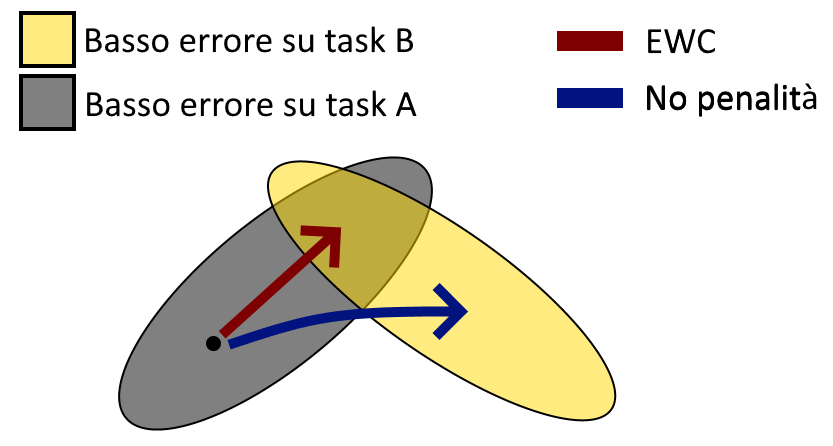
\includegraphics[width=0.5\textwidth]{img/ewc.png}
		\caption{Schematizzazione del comportamento di EWC}
		\label{fig:ewc}
	\end{center}
\end{figure}
% Implementazione: \cite{moriarty_ewc}
\subsection{Learning Without Forgetting}
La metodologia Learning Without Forgetting, delineata nell'omonima pubblicazione$^{\cite{li2017learning}}$, sfrutta esclusivamente i nuovi dati per addestrare il modello mantenendo la conoscenza già appresa.\\
Questo metodo parte da una rete che possiede parametri $\Theta$, di cui i parametri $\Theta_s$ sono condivisi fra i task e i parametri $\Theta_A$ sono specifici al task $A$. L'obiettivo è aggiungere parametri $\Theta_B$ per il nuovo task usando solo i nuovi dati senza deteriorare la conoscenza precedentemente appresa.\\\\
LWF inizia applicando il modello addestrato ai dati nuovi appena arrivati, registrando i risultati che esso produce. Dopodiché si addestra il modello, usando come loss la somma di due loss così definite:
\begin{equation}\label{eq:lwf_lossnew}
    loss_{new}(y_n, \overline{y}_n) = -y_n\cdot\log\overline{y}_n
\end{equation}
\begin{equation}\label{eq:lwf_lossnew}
    loss_{old}(y_o, \overline{y}_o) = -\sum_{i=1}^l y_o^{'(i)}\log y_o^{'(i)}
\end{equation}
dove
\begin{equation}\label{eq:lwf_lossnew}
    y_o^{'(i)} = \frac{\left(y_o^{(i)}\right)^{1/T}}{\sum_j \left(y_o^{(j)}\right)^{1/T}},\:\:\:\:\:
    \overline{y}_o^{'(i)} = \frac{\left(\overline{y}_o^{(i)}\right)^{1/T}}{\sum_j \left(\overline{y}_o^{(j)}\right)^{1/T}}
\end{equation}
$T$ è un parametro della \textit{Knowledge Distillation loss} settato a $T = 2$, $l$ è il numero di etichette, $y_n$ le etichette dei nuovi dati, $\overline{y}_n$ le predizioni dei nuovi dati, $y_o$ le precedenti previsioni del precedente modello e $\overline{y}_o$ le nuove previsioni del precedente modello.\\
La nuova loss è quindi
\begin{equation}\label{eq:lwf_loss}
    \lambda_o\cdot loss_{old}(Y_o, \overline{Y}_o) + loss_{new}(Y_n, \overline{Y}_n) + R(\Theta_s, \Theta_o, \Theta_n)
\end{equation}
Dove $\lambda_o$ è un peso che è tanto più grande quanto più sono importanti i vecchi dati rispetto ai nuovi, e $R$ è una funzione di regolarizzazione dei parametri.\\\\
Questa metodologia, che tiene di conto della performance che il modello aveva fino all'arrivo dei nuovi dati, tende quindi a mantenere la rete neurale simile a quella già addestrata, evitando così di variare considerevolmente i pesi distanziandoli da quelli appresi sui dati precedenti.
\section{Conclusione}
La scelta delle metodologie adottate, elemento centrale di questa tesi, si è rivelata particolarmente laboriosa. Anzitutto si è reso necessario inquadrare precisamente lo scopo del lavoro, cioè la comparazione fra diverse tecniche di addestramento continuo applicate a dati relativi allo human state monitoring. Questo ha richiesto la selezione di dataset appropriati e in seguito la scelta di semplici metodologie di addestramento continuo che potessero essere comparate. Il confronto ha quindi richiesto la ricerca e la scelta di metriche che ne misurassero i diversi aspetti di trasferimento della conoscenza e dell'accuratezza media e finale, oltre che i tempi di addestramento e la memoria utilizzata.\\
Il tutto è stato preceduto dalla ricerca e dallo studio personale dell'argomento, oltre che dalla scelta del linguaggio, delle librerie e dell'ambiente di sviluppo. Questo ha portato ad una lunga serie di esperimenti esplorativi, per poter studiare e testare i vari aspetti del machine learning e delle reti neurali prima, e dell'addestramento continuo successivamente. Questi esperimenti hanno permesso di affrontare le diverse problematiche comuni ad un problema di machine learning: il preprocessing dei dati, l'individuazione degli iperparametri adatti ad un modello, la corretta progettazione di una rete neurale, i tempi di addestramento e altri ancora.\\\\
Tutto questo lavoro è confluito in una serie di esperimenti finali che hanno prodotto i risultati presentati nel prossimo capitolo.

% Aggiungere queste parti? \/
% Esperimenti
% Magari racconto velocemente i diversi metodologie e difficoltà errori riscontrati?
% dovrei parlare di tutti i tentativi ed esperimenti da giugno a ora o solamente degli metodologie "finali" adottati?
% inizialmente: studio su come realizzare le reti neurali, esperimenti personali per familiarizzare con API
% poi inizio studio su come affrontare il training...

% --> capitolo successivo, Risultati  % background sugli approcci di continual learning usati
    \chapter{Risultati}
% Tabelle e grafici di ogni esperimento, con confronti fra i continual
\section{Risultati finali}
\paragraph{WESAD} Usando come modello due layer GRU da 18 unità, su WESAD sono stati ottenuti i seguenti risultati:

\begin{table}[h]
\footnotesize
    \begin{tabular}{l|c|c|c|c|c|c|c}
        \textbf{Scenario} & \textbf{Epoche} & \textbf{Tempo} & \textbf{Acc.} & \textbf{ACC} & \textbf{BWT} & \textbf{FWT} & \textbf{Memoria}\\
        \hline
        \textbf{Offline} & 28 & 94,69s & 99,07 & - & - & - & 2061,40 Mb\\
        \textbf{Continual} & 49,14$\pm$33,67 & 947,24s & 73,13$\pm$4,02 & 0,7721 & 0,0343 & 0,5397 & 2173 Mb\\
        \textbf{Cumulative} & 39,71$\pm$19,91 & 2786s & 81,97$\pm$8,67 & 0,961 & 0,1383 & 0,4674 & 2291,45 Mb\\
        \textbf{Replay} & 41,14$\pm$21,19 & 1063,51s & 78,29$\pm$3,32 & 0,7849 & -0,002 & 0,4582 & 2184,77 Mb\\
        \textbf{Episodic} & 35$\pm$26,26 & 1088,29s & 82,13$\pm$6,60 & 0,9095 & 0,0841 & 0,4226 & 2097,47 Mb\\
        \textbf{EWC} & 29,71$\pm$17,38 & 1342,81s & 70,74$\pm$4,74 & 0,7251 & 0,0113 & 0,4698 & 2187,40 Mb\\
        \textbf{LWF} & 44,29$\pm$18,30 & 3282,51s & 69,09$\pm$5,82 & 0,7419 & 0,0451 & 0,3248 & 2121,31 Mb\\
    \end{tabular}
    \caption{Risultati WESAD}
    \label{tab:reswesad}
\end{table}
\begin{figure}[h]
	\begin{center}
		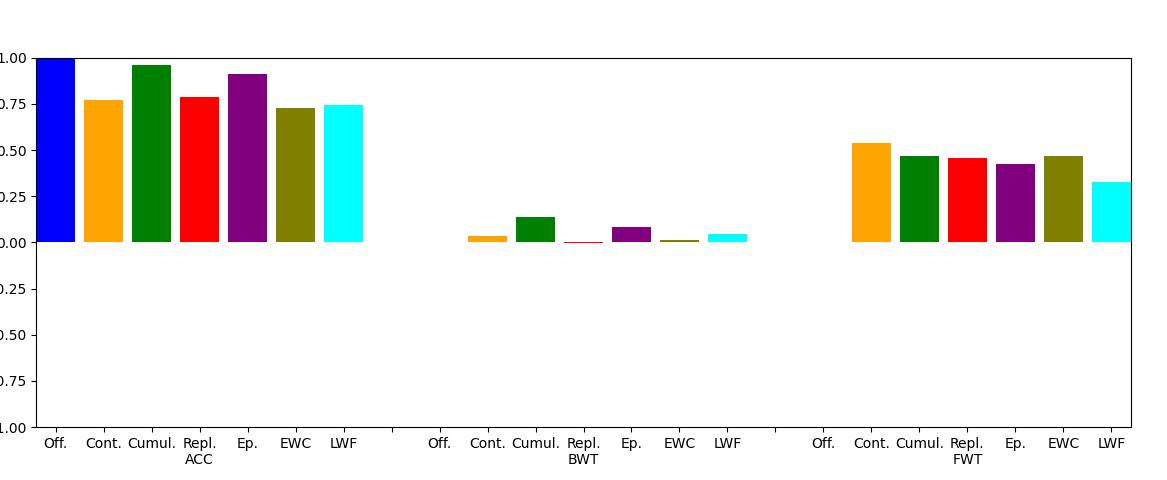
\includegraphics[width=0.95\textwidth]{img/graphs/wesad_final_metrics.png}
		\caption{Risultati su WESAD}
		\label{fig:wesad_metrics_graph}
	\end{center}
\end{figure}

L'accuratezza del 99\% raggiunta nel training offline dimostra come il dataset WESAD sia particolarmente adatto all'inferenza da parte di reti neurali ricorrenti dalla bassa complessità. Con poco più di 25 epoche di addestramento, abbiamo ottenuto un modello capace di classificare con un alto grado di accuratezza lo stato psico-fisico di un utente.\\
Ciò che è interessante notare è che l'accuratezza è mantenuta sopra il 70\% anche nella maggior parte degli approcci continual. La performance peggiore media la si ha nel \textit{Learning Without Forgetting}, che però ottiene comunque un'accuratezza finale (ACC) del 74\% e un FWT comunque ottimo. La miglior performance tra gli approcci continual è ottenuta dall'apprendimento cumulativo, con un'accuratezza finale del 96\% perfettamente paragonabile all'approccio offline, e in linea con la teoria. In tutti gli approcci, si ha un FWT elevato e molto superiore al BWT, segnale che ogni soggetto migliora molto l'apprendimento sui soggetti successivi, mentre non vi è particolare influenza sui precedenti soggetti o, se vi è, è positiva.\\\\
L'esperimento quindi dimostra come l'apprendimento continuo su dati sensoriali come respirazione, temperatura, elettrocardiogramma e simili possa portare a modelli con performance paragonabili all'apprendimento offline. Con un po' di \textit{fine-tuning} e \textit{model selection} con gli approcci continui si può probabilmente trovare un modello con performance ancora superiori a quelle sperimentate.
\begin{figure}[h]
	\begin{center}
		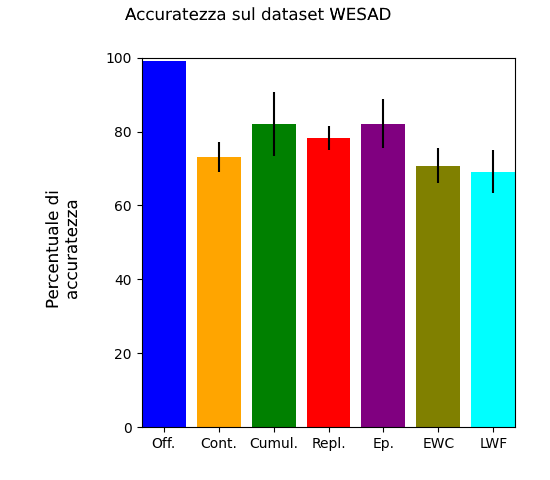
\includegraphics[width=0.5\textwidth]{img/graphs/wesad_final_accuracy.png}
		\caption{Accuratezza su WESAD}
		\label{fig:wesad_accuracy_graph}
	\end{center}
\end{figure}
\pagebreak
\paragraph{ASCERTAIN} Usando come modello due layer GRU da 24 unità, su ASCERTAIN sono stati raggiunti i seguenti risultati:
\begin{table}[h]
\footnotesize
    \begin{tabular}{l|c|c|c|c|c|c|c}
        \textbf{Scenario} & \textbf{Epoche} & \textbf{Tempo} & \textbf{Acc.} & \textbf{ACC} & \textbf{BWT} & \textbf{FWT} & \textbf{Memoria}\\
        \hline
         \textbf{Offline} & 3 & 29,14s & 42,78 & - & - & - & 1817,28 Mb\\
        \textbf{Continual} & 10,88$\pm$5,01 & 249,28s & 37,45$\pm$5,01 & 0,25 & -0,0168 & 0,0213 & 2154,36 Mb\\
        \textbf{Cumulative} & 9,25$\pm$6,81 & 932,56s & 39,06$\pm$4,26 & 0,2697 & 0,0064 & 0,0278 & 2297,17 Mb\\
        \textbf{Replay} & 13,25$\pm$10,03 & 402,96s & 39,48$\pm$4,37 & 0,2603 & -0,014 & 0,0485 & 2173,95 Mb\\
        \textbf{Episodic} & 12,62$\pm$7,94 & 498,24s & 38,80$\pm$4,04 & 0,2742 & 0,0048 & 0,0156 & 2231,42 Mb\\
        \textbf{EWC} & 24,14$\pm$16,94 & 810,96s & 36,08$\pm$5,66 & 0,2497 & -0,0183 & -0,0003 & 2171,62 Mb\\
        \textbf{LWF} & 21,62$\pm$10,20 & 879,68s & 35,69$\pm$5,43 & 0,2448 & 0.0327 & 0,0156 & 2103 Mb\\
    \end{tabular}
    \caption{Risultati ASCERTAIN}
    \label{tab:resascertain}
\end{table}
\begin{figure}[h]
	\begin{center}
		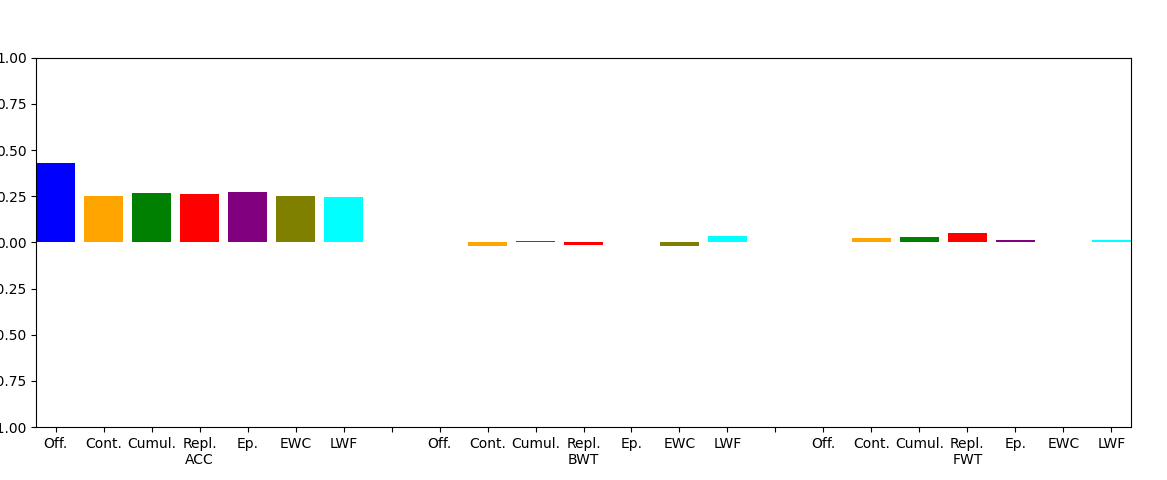
\includegraphics[width=0.95\textwidth]{img/graphs/ascertain_final_metrics.png}
		\caption{Risultati sul dataset ASCERTAIN}
		\label{fig:ascertain_metrics_graph}
	\end{center}
\end{figure}

Dall'approccio offline è subito chiaro come il dataset ASCERTAIN presenti una difficoltà maggiore rispetto a WESAD. In particolare, il dataset ASCERTAIN presenta dati particolarmente sbilanciati sulla classe 0 e informazioni riguardo le espressioni facciali dei soggetti durante l'esperimento. Questi dati sono di difficile classificazione.\\
Gli approcci continui sono comunque in linea con i risultati sul precedente dataset, con la performance peggiore ottenuta dal \textit{Learning Without Forgetting} mentre la migliore è ottenuta dall'approccio cumulativo grazie ad un BWT superiore all'approccio di replay. In molti casi si nota un trasferimento negativo di conoscenza all'indietro, sintomo di un lieve caso di \textit{catastrophic forgetting}.\\\\
Per poter dimostrare l'impatto dovuto allo sbilanciamento delle classi, il dataset ASCERTAIN è stato riorganizzato in soggetti "fittizi" come esposto di seguito.


\pagebreak
\paragraph{Custom ASCERTAIN} Dopo aver eseguito il preprocessing specificato precedentemente, tutti i dati di addestramento sono stati uniti in un unico insieme. Da questo insieme è stato estratto il test set, e il rimanente training set è stato suddiviso in 17 soggetti bilanciati da 108 sequenze di 160 punti ciascuno.\\
Usando come modello due layer GRU da 24 unità, su ASCERTAIN con i soggetti fittizi sono stati registrati i seguenti risultati:
\begin{table}[h]
\footnotesize
    \begin{tabular}{l|c|c|c|c|c|c|c}
        \textbf{Scenario} & \textbf{Epoche} & \textbf{Tempo} & \textbf{Acc.} & \textbf{ACC} & \textbf{BWT} & \textbf{FWT} & \textbf{Memoria}\\
        \hline
         \textbf{Offline} & 29 & 66,17s & 87,77 & - & - & - & 1945,91 Mb\\
        \textbf{Continual} & 7,75$\pm$5,33 & 226,24s & 87,01$\pm$0,64 & 0,2481 & -0,0241 & 0,0052 & 2143,71 Mb\\
        \textbf{Cumulative} & 7,25$\pm$8,80 & 872,8s & 87,66$\pm$0,16 & 0,2773 & 0,0032 & 0,0801 & 2273,07 Mb\\
        \textbf{Replay} & 12,125$\pm$12,94 & 299,52s & 87,13$\pm$0,75 & 0,2711 & -0,0012 & 0,306 & 2146,35 Mb\\
        \textbf{Episodic} & 5,5$\pm$3,94 & 319,76s & 82,19$\pm$3,95 & 0,339 & 0,0346 & 0,1043 & 2204,84 Mb\\
        \textbf{EWC} & 14,38$\pm$7,58 & 541,68s & 87,34$\pm$0,42 & 0,2467 & -0,0191 & 0,0845 & 2146,36 Mb\\
        \textbf{LWF} & 20,75$\pm$8,42 & 771,36s & 86,91$\pm$0,89 & 0,2495 & -0,0333 & -0,146 & 2095,93 Mb\\
    \end{tabular}
    \caption{Risultati su ASCERTAIN con soggetti fittizi bilanciati}
    \label{tab:rescustomascertain}
\end{table}
\begin{figure}[h]
	\begin{center}
		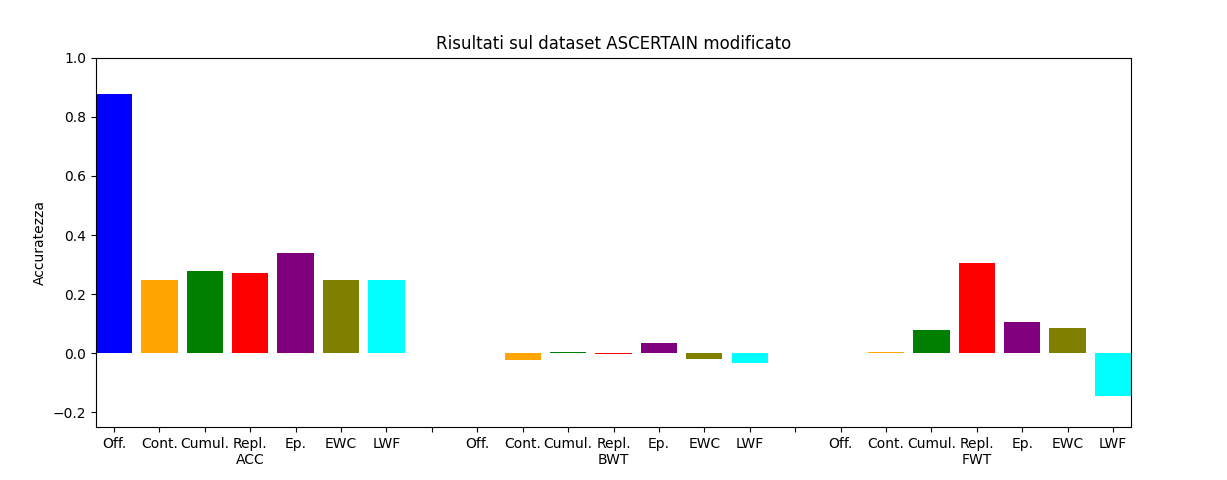
\includegraphics[width=0.95\textwidth]{img/graphs/customascertain_final_metrics.png}
		\caption{Risultati su ASCERTAIN con soggetti fittizi}
		\label{fig:customascertain_metrics_graph}
	\end{center}
\end{figure}

Dalla tabella \ref{tab:rescustomascertain} si evince subito come il bilanciamento abbia prodotto accuratezze medie molto superiori al dataset originale: l'approccio offline raggiunge l'87,77\% di accuratezza, paragonabile ai risultati ottenuti sul dataset WESAD, e gli approcci continui, in linea coi precedenti risultati, superano comunque l'80\% di accuratezza media in tutti i casi.\\
Dalle rimanenti metriche si nota comunque la difficoltà intrinseca del dataset, che raggiunge un'accuratezza finale del solo 33\% con l'approccio di replay episodico e BWT spesso negativo o comunque molto basso.
\begin{figure}[!tbp]
    \begin{minipage}[b]{0.5\textwidth}
		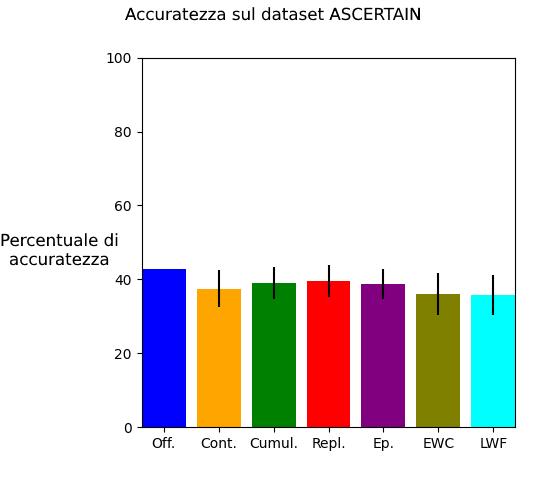
\includegraphics[width=\textwidth]{img/graphs/ascertain_final_accuracy.png}
		\caption{Accuratezza sul dataset ASCERTAIN originale}
		\label{fig:ascertain_accuracy_graph}
	\end{minipage}
    \hfill
    \begin{minipage}[b]{0.5\textwidth}
		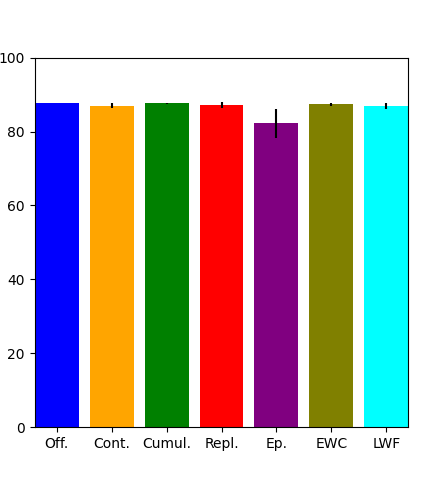
\includegraphics[width=\textwidth]{img/graphs/customascertain_final_accuracy.png}
		\caption{Accuratezza su ASCERTAIN con soggetti fittizi}
		\label{fig:customascertain_accuracy_graph}
	\end{minipage}
\end{figure}  % comparazione dei risultati con offline come baseline
    \chapter{Conclusioni}  % considerazioni sui risultati e applicabilità o meno delle strategie continual su HSM

    \backmatter
    \phantomsection
	\addcontentsline{toc}{chapter}{Bibliografia}
	\bibliography{Bibliografia}
	\bibliographystyle{siam}
	\chapter*{Ringraziamenti}
\markboth{RINGRAZIAMENTI}{}
\addcontentsline{toc}{chapter}{Ringraziamenti}
% Template tesi: Jacopo Belli, https://github.com/jacopobelli/Template-Tesi-UniPi
\cleardoublepage
\iffalse
\section{Introduzione}
Di seguito condivido, con più attenzione al contenuto che alla forma, i miei appunti di lavoro riguardo la tesi.
\pagebreak
\section{Dataset WESAD}
Il dataset, una volta scaricato, è stato ricampionato a 32Hz, ripulito dalle etichette 0, 4, 5, 6 e suddiviso in sottosequenze da 100 datapoint (equivalenti a 3s circa)
\begin{lstlisting}[language=Python]
import pickle
import numpy as np
import scipy.signal
import tensorflow.keras as keras

# Apertura del dataset WESAD
ds = {
    "S2": pickle.load(open("WESAD/S2/S2.pkl", 'rb'),
                      encoding='latin1'),
    # ...
    "S17": pickle.load(open("WESAD/S17/S17.pkl", 'rb'),
                      encoding='latin1')
}

for s in ds.keys():
    # Ricampionamento e concatenazione
    X = np.concatenate([
        scipy.signal.resample(ds[s]['signal']['chest']['ACC'],
                            len(ds[s]['signal']['wrist']['ACC'])),
        # ...
        scipy.signal.resample(ds[s]['signal']['wrist']['TEMP'],
                            len(ds[s]['signal']['wrist']['ACC']))
        ], axis = 1)
    Y = scipy.signal.resample(ds[s]['label'],
                            len(ds[s]['signal']['wrist']['ACC']))
    # Standardizzazione
    X = (X - X.mean(axis = 0)) / X.std(axis = 0)
    Y = np.around(Y)
    Y = abs(Y.astype(np.int32))
    
    # Pulizia
    X = X[(Y>0) & (Y<5)]
    Y = Y[(Y>0) & (Y<5)]
    
    # Sottosequenze
    count = 0
    prev = Y[0]
    LenSubsequences = []
    for elem in Y:
        if(elem != prev):
            LenSubsequences.append(count)
            count = 0
        count += 1
        prev = elem
    SubsequencesX = []
    SubsequencesY = []
    i = 0
    for elem in LenSubsequences:
        for j in range(0, elem, 100):
            if(j+100 <= elem):
                SubsequencesX.append(X[i+j:i+j+100])
                SubsequencesY.append(Y[i+j+50])
        i += elem
    
    # Reshape
    X_WES = (np.array(SubsequencesX, dtype = np.float64))
            .reshape(-1, 100, 14)
    Y = np.array(SubsequencesY, dtype = np.float32) - 1
    y_WES = keras.utils.to_categorical(Y, num_classes = 4)
    
    # Salvataggio soggetto
    with open("WESAD/splitted/X" + s + ".pkl", 'wb') as handle:
        pickle.dump(X_WES, handle, protocol=pickle.HIGHEST_PROTOCOL)
    with open("WESAD/splitted/y" + s + ".pkl", 'wb') as handle:
        pickle.dump(y_WES, handle, protocol=pickle.HIGHEST_PROTOCOL)
\end{lstlisting}
I dati li ho lasciati divisi per soggetto, e di ogni label inizialmente sono state prese 1600 istanze, successivamente tutte (come nel codice riportato).
Il risultato sono dataset da circa 1000 sottosequenze di 100 istanze, con 14 feature ciascuna.
\pagebreak
\section{Dataset ASCERTAIN}
Il codice, presente in\\\texttt{https://teaching-gitlab.di.unipi.it/f.matteoni/thesis-code/-/blob/master/ascertain\_data.py}, è stato realizzato seguendo il notebook RNN\_benchmarking\_1\_layer.ipynb nella repository di Daniele Di Sarli.\\
Il dataset è preparato componendo le 4 classi (0 = arousal $>$ 3 $\wedge$ valence $>$ 0, 1 = arousal $>$ 3 $\wedge$ valence $\leq$ 0, 2 = arousal $\leq$ 3 $\wedge$ valence $>$ 0, 3 = arousal $\leq$ 3 $\wedge$ valence $\leq$ 0), ricampionato a 32 Hz, pulito da valori nulli e/o mancanti, standardizzato con media = 0 e deviazione standard = 1 e ogni soggetto è stato preparato unendo le 17 features su un solo asse. Le sequenze sono state realizzate di 160 datapoint: inizialmente le realizzai di 100 come per WESAD ma i risultati erano inferiori (seppur di poco) all'utilizzo di sequenze di 160.
\section{Continual learning}
\subsection{Primo test}
\paragraph{Modello} Un layer GRU con 29 unità, e un layer output Dense da 4 unità con attivazione softmax e regolarizzazione:
\begin{lstlisting}[language=Python]
model = tf.keras.models.Sequential()
model.add(tf.keras.layers.GRU(29, input_shape=(100, 14)))
model.add(tf.keras.layers.Dense(4, activation = 'softmax',
          kernel_regularizer = 
              tf.keras.regularizers.l1_l2(l1 = 1e-5, l2 = 1e-5),
          bias_regularizer = 
              tf.keras.regularizers.l1_l2(l1 = 1e-5, l2 = 1e-5),
          activity_regularizer = 
              tf.keras.regularizers.l1_l2(l1 = 1e-6, l2 = 1e-6)))
\end{lstlisting}
Il modello è compilato con la \texttt{categorical\_crossentropy} come loss, Adam con learning rate $= 0.005$, $\beta_1 = 0.85$ e $\beta_2 = 0.999$ come optimizer e accuracy come metrica.
\paragraph{Scenari}
\begin{itemize}
    \item[] \textbf{Dataset completo}, cioè tutti i soggetti concatenati assieme in un unico training set.
    \item[] \textbf{Continual training}, cioè un training eseguito a coppia di soggetti, e tra ogni coppia
    \item[] \textbf{Cumulative training}, cioè un training eseguito a coppia di soggetti come nel continual ma man mano "sommiamo" i soggetti in modo da avere ad ogni passo anche tutti i precedenti
\end{itemize}
\paragraph{Risultati} Il training è stato eseguito su training set diverso a seconda dello scenario, ma sempre usando S17 come soggetto di test.\\\\
\begin{tabular}{l|c|c|c|c}
    \textbf{Scenario} & \textbf{Media epoche} & \textbf{Std. Dev.} & \textbf{Media Accuracy} & \textbf{Std. Dev} \\
    \hline 
    \textbf{Offline} & 17 & 0 & 28.57\% & 0 \\
    \textbf{Continual} & 60 & 0 & \textbf{45.15\%} & 16.33 \\
    \textbf{Cumulative} & 66.29 & 36.79 & 39.54\% & 12.46 \\
\end{tabular}
\begin{figure}
    \centering
    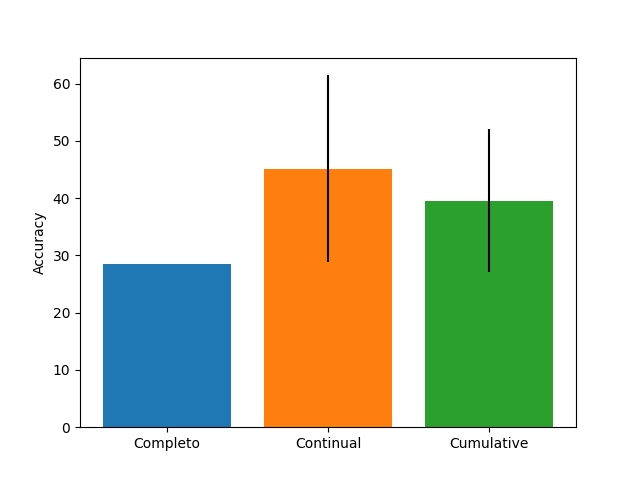
\includegraphics[scale=0.75]{img/first.png}
    \caption{Accuracy nel primo test}
    \label{fig:first}
\end{figure}
\subsection{Secondo test}
\paragraph{Modello} Il modello è simile al precedente ma con due layer GRU da 30 unità: questo è il risultato di una gridsearch.
\paragraph{Risultati} Di seguito\\
\begin{tabular}{l|c|c|c|c}
    \textbf{Scenario} & \textbf{Media epoche} & \textbf{Std. Dev.} & \textbf{Media Accuracy} & \textbf{Std. Dev} \\
    \hline 
    \textbf{Offline} & 100 & 0 & 30.36\% & 0 \\
    \textbf{Continual} & 100 & 0 & \textbf{46.17\%} & 12.50 \\
\end{tabular}
\begin{figure}
    \centering
    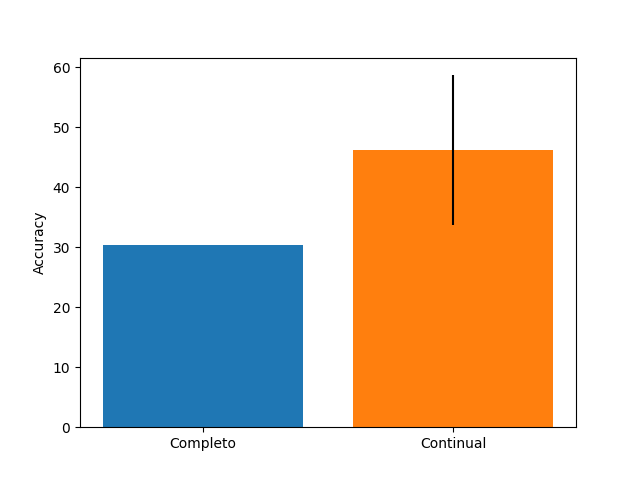
\includegraphics[scale=0.75]{img/second.png}
    \caption{Accuracy nel secondo test}
    \label{fig:second}
\end{figure}
Notando un'accuracy del 100\% sia su training set che su validation set, ho giudicato il modello inadatto per overfitting. Ho quindi deciso di cambiare dataset, prendendo tutte le istanze di ogni label.
\paragraph{Risultati} Con il nuovo dataset più capiente ho ottenuto risultati migliori\\
\begin{tabular}{l|c|c|c|c}
    \textbf{Scenario} & \textbf{Media epoche} & \textbf{Std. Dev.} & \textbf{Media Accuracy} & \textbf{Std. Dev} \\
    \hline 
    \textbf{Offline} & 9 & 0 & \textbf{56.24\%} & 0 \\
    \textbf{Continual} & 79.29 & 35.11 & 53.72\% & 14.24\\
\end{tabular}
\begin{figure}
    \centering
    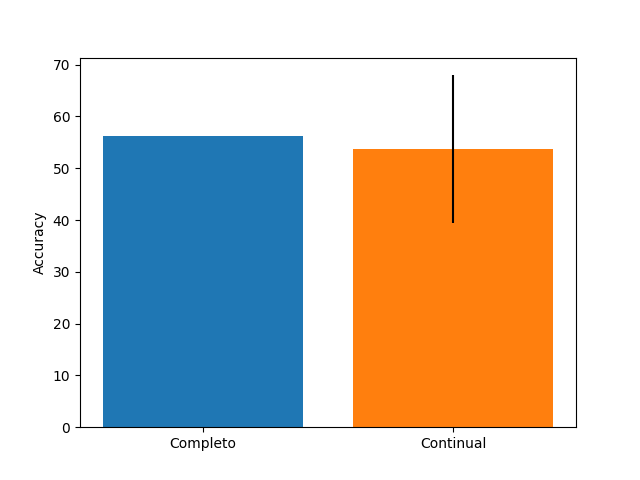
\includegraphics{\includegraphics[scale=0.75]{img/second2.png}}
    \caption{Risultati con il nuovo dataset}
    \label{fig:second2}
\end{figure}
\subsection{Terzo test}
\paragraph{Modello} Questo test l'ho eseguito sostituendo LSTM a GRU nel modello, cioè rimanendo con due layer da 30 unità più l'output layer Dense da 4 unità softmax.\\
Ho notato che un "replay" ingenuo, ovvero il portarsi dietro tutti i soggetti già usati nel training all'interno del training set successivo sommandoli con i due soggetti "nuovi", migliora di molto l'accuracy su S17. Ho quindi provato una tecnica di replay più snella: mantenere di volta in volta il 25\% casuale dei datapoint del trainingset attuale.
\paragraph{Risultati} Di seguito\\
\begin{tabular}{l|c|c|c|c}
    \textbf{Scenario} & \textbf{Media epoche} & \textbf{Std. Dev.} & \textbf{Media Accuracy} & \textbf{Std. Dev} \\
    \hline 
    \textbf{Offline} & 11 & 0 & 59.59\% & 0 \\
    \textbf{Continual} & 58.29 & 48.17 & 50.70\% & 8.24\%\\
    \textbf{Cumulative} & 26.43 & 32.20 & \textbf{62.83\%} & 8.20\%\\
    \textbf{Replay 25\%} & 17.43 & 11.32 & 61.07\% & 4.77\%\\
\end{tabular}
\begin{figure}
    \centering
    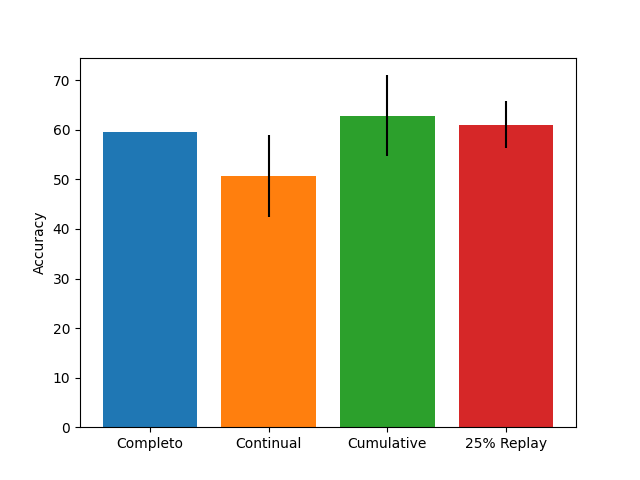
\includegraphics[scale=0.75]{img/third.png}
    \caption{Risultati nel terzo test}
    \label{fig:third}
\end{figure}
\pagebreak
\subsection{Quarto Test}
\paragraph{Scenario} A questo punto ho voluto provare una serie di modelli diversi sulla nuova tecnica, il replay training.
\paragraph{Risultati} Di seguito\\
\begin{tabular}{l|c|c|c|c}
    \textbf{Modello} & \textbf{Media epoche} & \textbf{Std. Dev.} & \textbf{Media Accuracy} & \textbf{Std. Dev} \\
    \hline 
    \textbf{Un layer LSTM con 30 unità} & 11.71 & 6.13 & \textbf{70.59\%} & 12.17\% \\
    \textbf{Un layer LSTM con 29 unità} & 12 & 10 & 52.33\% & 6.14\%\\
    \textbf{Un layer LSTM con 25 unità} & 21 & 8.59 & 58.72\% & 4.14\%\\
    \textbf{Un layer LSTM con 15 unità} & 28.14 & 24.03 & 59.88\% & 3.44\%\\
\end{tabular}
\begin{figure}
    \centering
    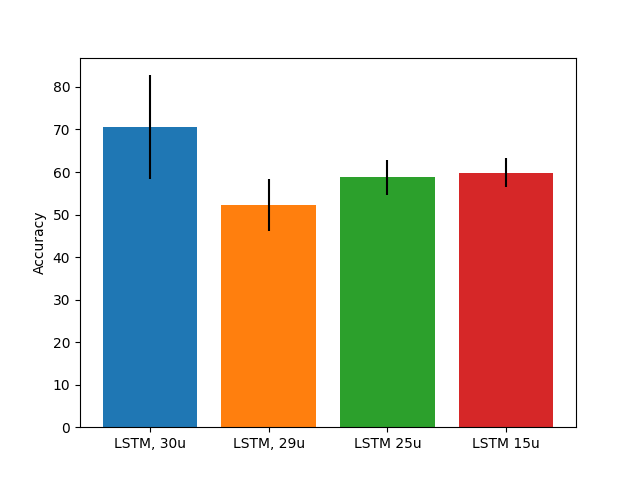
\includegraphics[scale=0.75]{img/fourth.png}
    \caption{Confronto fra modelli LSTM}
    \label{fig:fourth}
\end{figure}

\subsection{Quinto test}
\paragraph{Scenario} Stesso cambio di modello ma con GRU
\paragraph{Risultati} Di seguito\\
\begin{tabular}{l|c|c|c|c}
    \textbf{Modello} & \textbf{Media epoche} & \textbf{Std. Dev.} & \textbf{Media Accuracy} & \textbf{Std. Dev} \\
    \hline 
    \textbf{Un layer GRU con 30 unità} & 49.29 & 43.05 & \textbf{59.80\%} & 3.98\% \\
    \textbf{Due layer GRU con 30 unità} & 45 & 29.44 & 59.71\% & 3.27\%\\
\end{tabular}
\begin{figure}
    \centering
    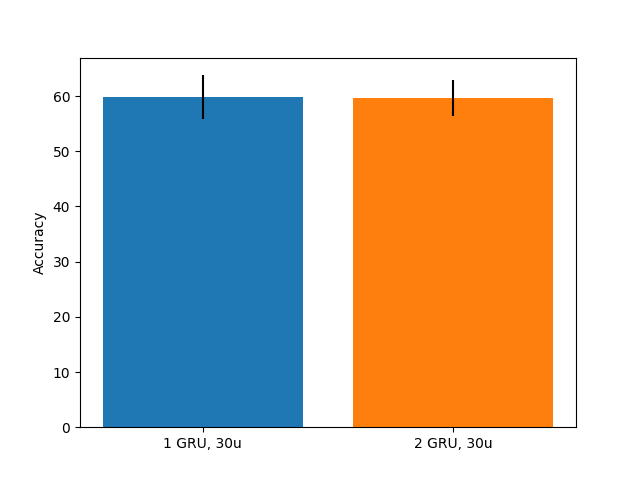
\includegraphics[scale=0.75]{img/fifth.png}
    \caption{Confronto fra modelli GRU}
    \label{fig:fifth}
\end{figure}
\subsection{Sesto Test}
\paragraph{Scenario} Ho quindi deciso di fare un test comparativo fra le varie tecniche scegliendo come modello quello da un singolo layer GRU da 30 unità.
Il test, automatizzato in un singolo script, prevede:
\begin{itemize}
    \item \textbf{total training}: soggetti S2-S16 insieme, test su S17
    \item \textbf{continual training}: soggetti S2-S3, test su S17, riprendo training con S4-S5, test e così via
    \item \textbf{cumulative training}: soggett S2-S3, test su S17, aggiungo S4-S5 al tr set, test su S17 e così via
    \item \textbf{replay training}: soggetti S2-S3, test su S17, mantengo il 25\% del tr set e aggiungo S4-S5, test e così via
\end{itemize}
\paragraph{Risultati} Di seguito\\
\begin{tabular}{l|c|c|c|c}
    \textbf{Scenario} & \textbf{Media epoche} & \textbf{Std. Dev.} & \textbf{Media Accuracy} & \textbf{Std. Dev} \\
    \hline 
    \textbf{Offline} & 14 & 0 & 65.35\% & 0\% \\
    \textbf{Continual} & 72.29 & 43.83 & 52.57\% & 8.51\%\\
    \textbf{Cumulative} & 18.71 & 33.32 & 59.18\% & 2.16\%\\
    \textbf{Replay} & 35.71 & 41.13 & \textbf{65.13\%} & 8.74\%\\
\end{tabular}
\begin{figure}
    \centering
    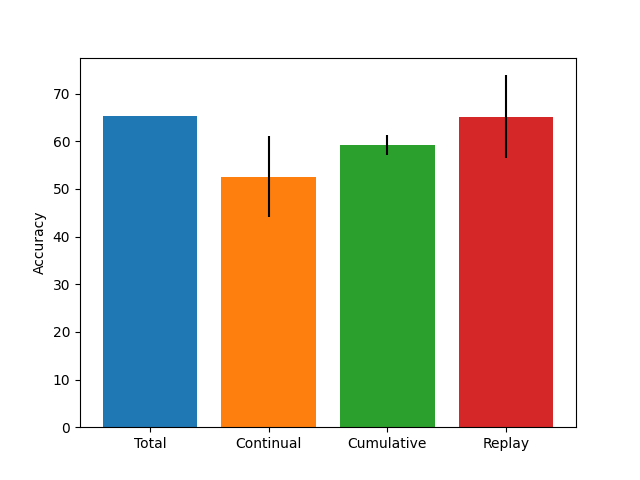
\includegraphics[scale=0.75]{img/sixth.png}
    \caption{Confronto fra scenari}
    \label{fig:sixth}
\end{figure}
Ulteriore conferma di un risultato teorico: mantenere esempi già addestrati mitiga il catastrophic forgetting.\\\\
Nel caso del continual training senza ripetizioni, si ha una costante diminuzione dell'accuracy su S17 che è sintomo di catastrophic forgetting.\\
\begin{figure}
    \centering
    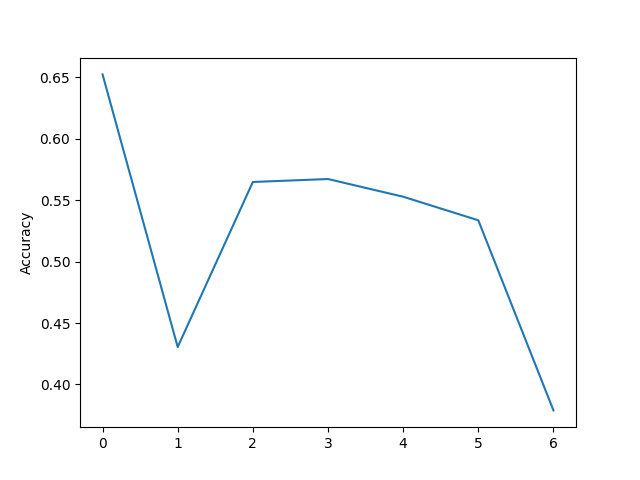
\includegraphics[scale=0.5]{img/cont6.png}
    \caption{Andamento accuracy del continual learning}
    \label{fig:cont6}
\end{figure}
Mentre il cumulative training suppongo vada in overfitting per i troppi dati.\\
\begin{figure}
    \centering
    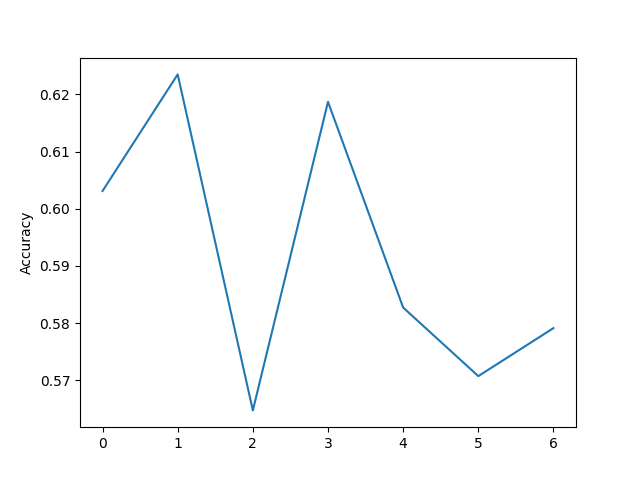
\includegraphics[scale=0.5]{img/sum6.png}
    \caption{Andamento accuracy del cumulative learning}
    \label{fig:sum6}
\end{figure}
Replay, d'altro canto, si comporta al pari del total training, pur mantenendo di coppia in coppia solo il 25\% dei dati dei soggetti precedenti.\\
\begin{figure}
    \centering
    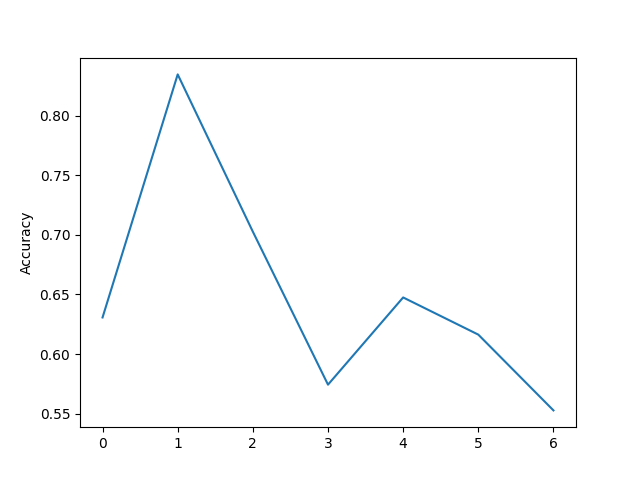
\includegraphics[scale=0.5]{img/repl6.png}
    \caption{Andamento accuracy del replay learning}
    \label{fig:repl6}
\end{figure}
\subsection{Settimo test}
\paragraph{Scenario} Vedendo come si comporta bene il replay, ho deciso di provare diverse tecniche di replay. Il modello è un layer singolo GRU da 30 unità, più quello output solito.
\begin{itemize}
    \item[] \textbf{Baseline}: tecnica usata fin'ora ma mantenendo solo il 10\% dei dati
    \item[] \textbf{25\%}: cioè mantengo il 25\% dei dati
    \item[] \textbf{Memoria episodica}, mantenendo $m = 50$ istanze a caso per ogni label
    \item[] \textbf{Memoria episodica}, mantenendo $m = 50$ \textit{predizioni} per ogni label
\end{itemize}
\paragraph{Risultati} Di seguito\\
\begin{tabular}{l|c|c|c|c}
    \textbf{Scenario} & \textbf{Media epoche} & \textbf{Std. Dev.} & \textbf{Media Accuracy} & \textbf{Std. Dev} \\
    \hline 
    \textbf{Replay 10\%} & 58.43 & 35.66 & 51.54\% & 8.53\% \\
    \textbf{Replay 25\%} & 42.71 & 39.88 & 55.69\% & 8.12\%\\
    \textbf{$m = 50$ istanze} & 45.43 & 41.74 & 56.46\% & 4.44\%\\
    \textbf{$m = 50$ previsioni} & 23 & 32.16 & \textbf{57.01\%} & 6.02\%\\
\end{tabular}
\begin{figure}
    \centering
    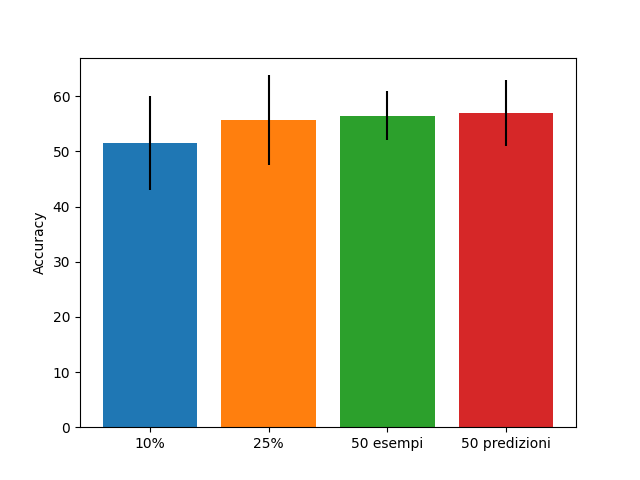
\includegraphics[scale=0.75]{img/seventh.png}
    \caption{Confronto tecniche su GRU}
    \label{fig:seventh}
\end{figure}
\subsection{Ottavo test}
\paragraph{Scenario} Stesso scenario precedente ma il modello è un layer singolo LSTM da 30 unità, più quello output solito.
\paragraph{Risultati} Di seguito\\
\begin{tabular}{l|c|c|c|c}
    \textbf{Scenario} & \textbf{Media epoche} & \textbf{Std. Dev.} & \textbf{Media Accuracy} & \textbf{Std. Dev} \\
    \hline 
    \textbf{Replay 10\%} & 26.71 & 25.63 & 53.25\% & 9.55\% \\
    \textbf{Replay 25\%} & 51.71 & 40.31 & 61.34\% & 7.22\%\\
    \textbf{$m = 50$ istanze} & 24 & 17.74 & \textbf{62.63\%} & 8.44\%\\
    \textbf{$m = 50$ previsioni} & 40.43 & 34.50 & 54.40\% & 7.44\%\\
\end{tabular}
\begin{figure}[h]
    \centering
    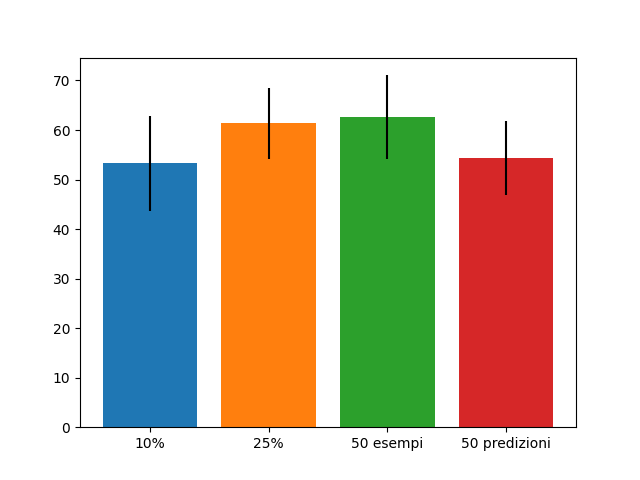
\includegraphics[scale=0.75]{img/eigth.png}
    \caption{Confronto tecniche su LSTM}
    \label{fig:eigth}
\end{figure}
\subsection{Nono test}
\paragraph{Scenario} Questa volta volevo confrontare l'uso di un modello con LSTM e l'uso di un modello con GRU, entrambi con un layer del rispettivo tipo con 30 unità e il solito layer output Dense da 4 unità softmax.
\paragraph{Risultati LSTM} Di seguito\\
\begin{figure}[h]
    \centering
    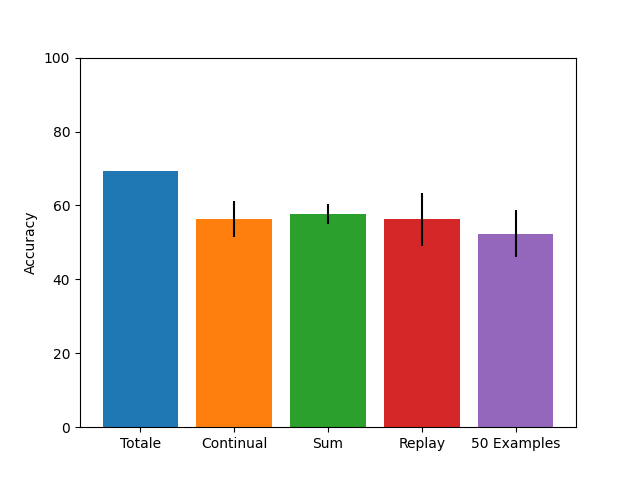
\includegraphics[scale=0.75]{img/autotest_LSTM.png}
    \caption{Risultati LSTM}
    \label{fig:autotest_LSTM}
\end{figure}
\begin{tabular}{l|c|c|c|c}
    \textbf{Scenario} & \textbf{Media epoche} & \textbf{Std. Dev.} & \textbf{Media Accuracy} & \textbf{Std. Dev} \\
    \hline 
    \textbf{Offline} & 19 & 0 &\textbf{ 59.42\%} & 0\% \\
    \textbf{Continual} & 37.43 & 33.77 & 56.35\% & 4.97\%\\
    \textbf{Cumulative} & 28.14 & 30.79 & 57.59\% & 2.60\%\\
    \textbf{Replay 25\%} & 19.43 & 16.92 & 56.22\% & 6.32\%\\
    \textbf{$m = 50$ istanze} & 20.71 & 32.69 & 52.33\% & 6.32\%\\
\end{tabular}
\paragraph{Risultati GRU} Di seguito\\
\begin{figure}[h]
    \centering
    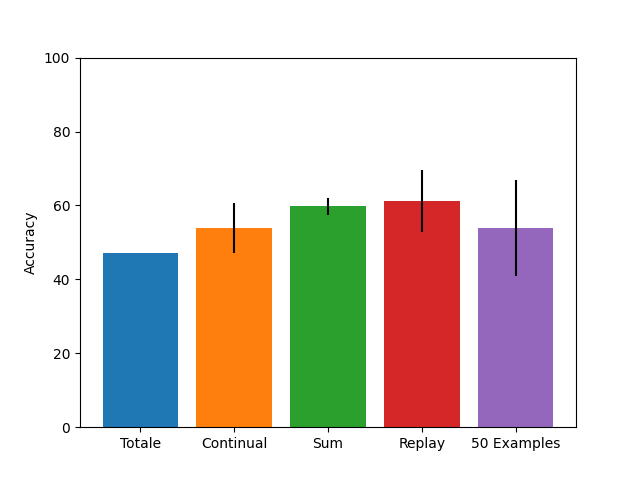
\includegraphics[scale=0.75]{img/autotest_GRU.png}
    \caption{Risultati GRU}
    \label{fig:autotest_GRU1}
\end{figure}
\begin{tabular}{l|c|c|c|c}
    \textbf{Scenario} & \textbf{Media epoche} & \textbf{Std. Dev.} & \textbf{Media Accuracy} & \textbf{Std. Dev} \\
    \hline 
    \textbf{Offline} & 16 & 0 & 47.24\% & 0\% \\
    \textbf{Continual} & 86.14 & 33.94 & 53.80\% & 6.77\%\\
    \textbf{Cumulative} & 27.43 & 33.12 & 59.75\% & 2.35\%\\
    \textbf{Replay 25\%} & 39.14 & 34.27 & \textbf{61.24\%} & 8.33\%\\
    \textbf{$m = 50$ istanze} & 41.14 & 37.23 & 53.91\% & 13.10\%\\
\end{tabular}
Le strategie "continual" si comportano meglio con GRU, mentre LSTM funziona meglio sul training offline.

\subsection{Decimo test}
\paragraph{Scenario} Ho provato il modello da 1 layer GRU da 30 unità con diversi valori di $m$ sul replay episodico
\paragraph{Risultati} Di seguito\\
\begin{figure}[h]
    \centering
    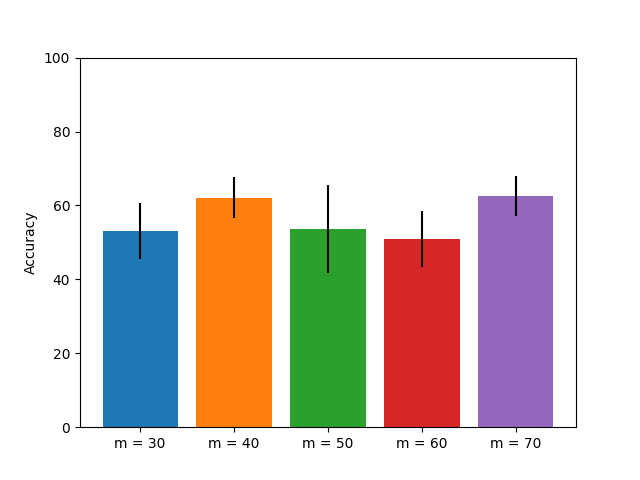
\includegraphics[scale=0.75]{img/episodic_m_test.png}
    \caption{Risultati}
    \label{fig:episodic_m_test}
\end{figure}
\begin{tabular}{l|c|c|c|c}
    \textbf{$m =$} & \textbf{Media epoche} & \textbf{Std. Dev.} & \textbf{Media Accuracy} & \textbf{Std. Dev} \\
    \hline 
    \textbf{30} & 54 & 40.07 & 53.17\% & 7.57\% \\
    \textbf{40} & 61.14 & 44.20 & 62.09\% & 5.60\%\\
    \textbf{50} & 39.14 & 42.80 & 53.61\% & 11.98\%\\
    \textbf{60} & 66.57 & 33.91 & 50.91\% & 7.57\%\\
    \textbf{70} & 43.14 & 40.35 & \textbf{62.56\%} & 5.43\%\\
\end{tabular}
\pagebreak
\subsection{Undicesimo test}
\paragraph{Obiettivo} Vorrei provare a inquadrare metriche utili a comparare i vari approcci al continual learning, in particolare poter misurare il catastrophic forgetting e il backward/forward transfer. Ho trovato, nel paper che descrive l'approccio Gradient Episodic Memory, tre metriche utili:
\begin{itemize}
    \item[\textbf{ACC}] Average accuracy = $\frac{1}{T}\sum_{i=1}^T R_{T,i}$\\
    Con questa matrica si misura l'accuratezza generale del modello.
    \item[\textbf{BWT}] Backward transfer = $\frac{1}{T-1}\sum_{i=1}^{T-1} R_{T,i} - R_{i,i}$\\
    Viene misurato l'impatto che l'apprendimento ha avuto su tutti i task precedenti.
    \item[\textbf{FWT}] Forward transfer = $\frac{1}{T-1}\sum_{i=2}^T R_{i-1,i} - b_i$\\
    Viene misurato quanto è migliorato l'apprendimento sul finale rispetto all'inizializzazione casuale iniziale.
\end{itemize}
Dove con $T$ indichiamo il numero di task, $R \in R^{T\times T}$ è la matrice delle accuratezze: dopo che il modello ha appreso il task $t_i$, valutiamo la sua performance su tutti i $T$ task. Quindi $R_{i,j}$ è la performance del modello sul task $t_j$ dopo aver osservato l'ultima istanza del task $t_i$.\\
$b$ è il vettore delle accuratezze per ogni task all'inizializzazione casuale.
\paragraph{Implementazione} Ho implementato seguendo questa filosofia: ogni classe è un "task", e a fine apprendimento su una coppia si aggiorna $R$ in base .\\
Ho quindi innanzitutto diviso il test set per task:
\begin{lstlisting}[language = Python]
Xts = pickle.load(open("WESAD/splitted/XS17_disarli.pkl", 'rb'), encoding='latin1')
yts = pickle.load(open("WESAD/splitted/yS17_disarli.pkl", 'rb'), encoding='latin1')

Xts_1, Xts_2, Xts_3, Xts_4, yts_1, yts_2, yts_3, yts_4 =
    [], [], [], [], [], [], [], []
idx_1 = [i for i, x in enumerate(yts) if x[0] == 1]
for i in idx_1:
    Xts_1.append(Xts[i])
    yts_1.append([1., 0., 0., 0.])
Xts_1, yts_1 = np.array(Xts_1), np.array(yts_1)
# ...
idx_4 = [i for i, x in enumerate(yts) if x[3] == 1]
for i in idx_4:
    Xts_4.append(Xts[i])
    yts_4.append([0., 0., 0., 1.])
Xts_4, yts_4 = np.array(Xts_4), np.array(yts_4)
\end{lstlisting}
\pagebreak
Subito dopo aver compilato il modello, preparo le metriche e inizializzo $b$:
\begin{lstlisting}[language = Python]
R = []
T = 4
b = [model.evaluate(Xts_1, yts_1)[1],
     model.evaluate(Xts_2, yts_2)[1],
     model.evaluate(Xts_3, yts_3)[1],
     model.evaluate(Xts_4, yts_4)[1]]
ACC, BWT, FWT = 0, 0, 0
\end{lstlisting}
Durante l'apprendimento, oltre a valutare sul test set intero popolo anche $R$:
\begin{lstlisting}[language = Python]
R.append([model.evaluate(Xts_1, yts_1)[1],
          model.evaluate(Xts_2, yts_2)[1],
          model.evaluate(Xts_3, yts_3)[1],
          model.evaluate(Xts_4, yts_4)[1]])
\end{lstlisting}
A fine allenamento calcolo le metriche finali (codice temporaneo):
\begin{lstlisting}[language = Python]
t = 0
for i in range(T):
        t += R[T-1][i]
ACC = t/T

t = 0
for i in range(T-1):
        t += (R[T-1][i] - R[i][i])
BWT = t/(T-1)

t = 0
for i in range(1, T):
        t += (R[i-1][i] - b[i])
FWT = t/(T-1)
\end{lstlisting}
\pagebreak
\paragraph{Risultati} Ho provato le metriche su tre scenari di continual learning diversi:
\begin{tabular}{l|c|c|c|c|c}
    \textbf{Scenario} & \textbf{Epoche} & \textbf{Accuracy} & \textbf{ACC} & \textbf{BWT} & \textbf{FWT} \\
    \hline 
    \textbf{$m = 70$} & 20.29$\pm$16.21 & 59.82\%$\pm$5.95\% & 0.4665 & -0.0202 & 0.4069 \\
    \textbf{Replay 10\%} & 46.14$\pm$42.93 & 59.58\%$\pm$13.83\% & 0.4745 & -0.1617 & 0.5320\\
    \textbf{Continual} & 48.29$\pm$37.38 & 46.44\%$\pm$11.35\% & 0.4813 & -0.0242 & 0.0481\\
\end{tabular}\\\\
L'approccio episodic (cioè replay di un numero $m$ di memorie per ogni classe/task) e quello replay (cioè replay di una percentuale del training set) hanno accuratezza sul test set sempre molto comparabili, se non adirittura simili, ma con queste ultime metriche si nota come il replay abbia durante l'apprendimento un impatto molto più grande sia sul backward transfer che sul forward transfer.\\
BWT negativo in tutti e tre i casi, ma in particolare modo nel replay, indica l'influenza negativa che si ha in generale sui task precedenti all'apprendimento di un nuovo task (cioè un elevato catastrophic forgetting).\\
FWT positivo invece indica l'influenza positiva che apprendere un task corrente ha sulla performance dei futuri task. In particolare, un FWT alto indica la capacità del modello di effettuare un apprendimento "zero-shot", cioè di apprendere un task successivo semplicemente sfruttando la struttura dei task già appresi (ed è il caso del test effettuato, avendo ad ogni passo coppie di soggetti dove sono presenti tutti i task da apprendere che quindi influenzano positivamente l'apprendimento sulle coppie successive).\\
\begin{figure}[h]
    \centering
    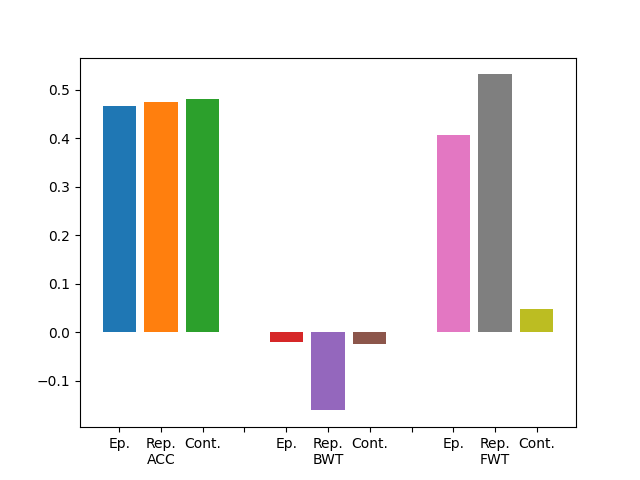
\includegraphics[scale=0.75]{img/accbwtfwt.png}
    \caption{Risultati}
    \label{fig:accbwtfwt}
\end{figure}
\begin{figure}[h]
    \centering
    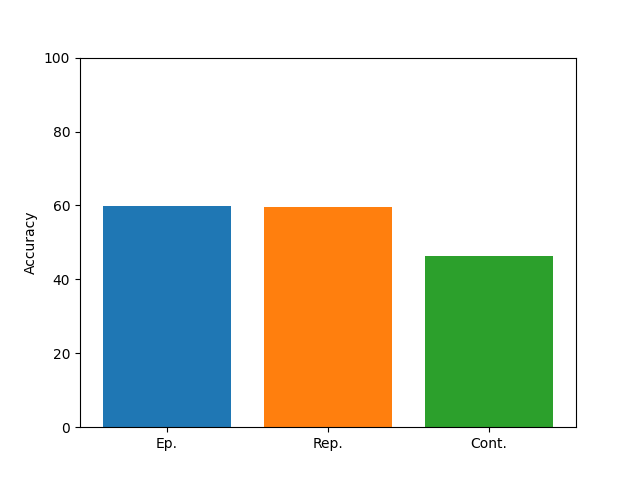
\includegraphics[scale=0.75]{img/accbwtfwt_accuracy.png}
    \caption{Accuracy}
    \label{fig:accbwtfwt_accuracy}
\end{figure}
\subsection{Dodicesimo test}
\paragraph{Obiettivo} Vedere come si comportano i vari approcci visti fin'ora ma su un modello che impara un task per volta, invece che a coppie di soggetti con tutti i task. Il test verrà fatto sempre su S17. Per prima cosa dividerò il dataset per classe, anziché per soggetto.\\
In futuro vorrei provare altri modelli, altre tecniche di replay.
\paragraph{Risultati} Di seguito i risultati raccolti
\begin{figure}[h]
    \centering
    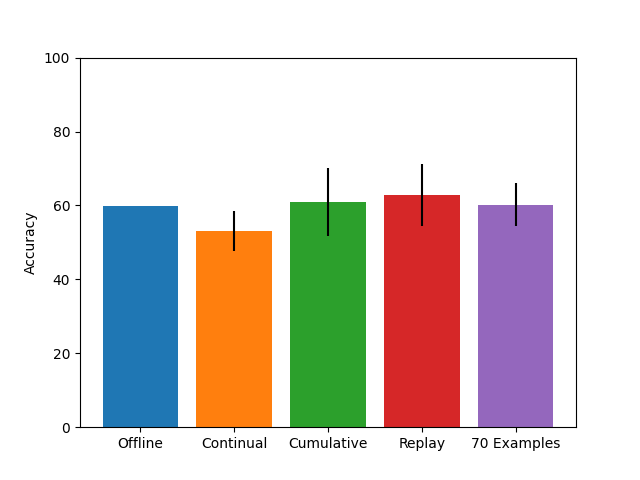
\includegraphics[scale=0.75]{img/autotest_20210701/autotest_GRU.png}
    \caption{Learning a coppia di soggetti}
    \label{fig:autotest_GRU}
\end{figure}
\begin{figure}[h]
    \centering
    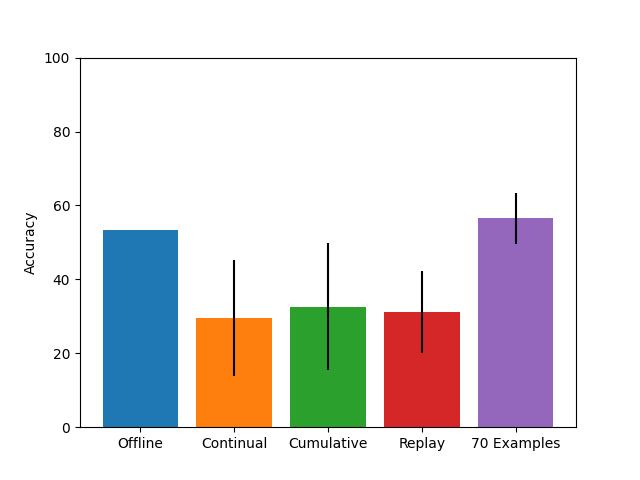
\includegraphics[scale=0.75]{img/autotest_20210701/autotest_task_GRU.png}
    \caption{Learning task per task}
    \label{fig:autotest_task_GRU}
\end{figure}
\begin{figure}[h]
    \centering
    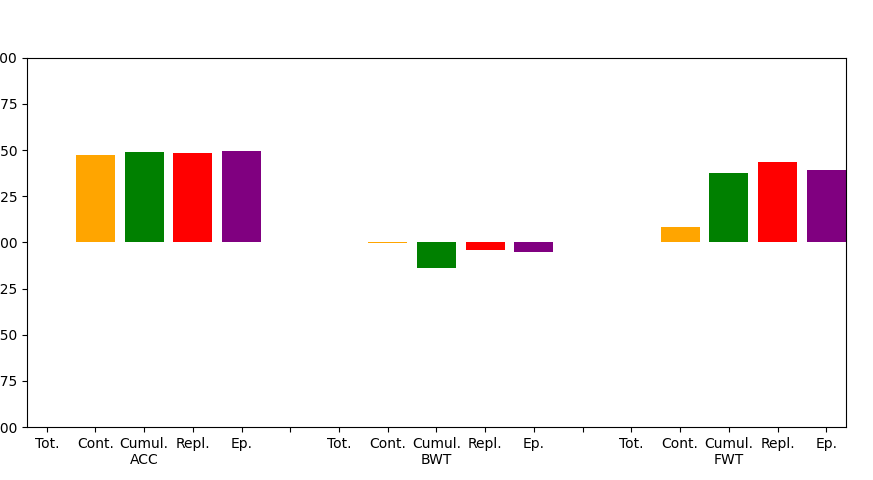
\includegraphics[scale=0.6]{img/autotest_20210701/autotest_GRU_accbwtfwt.png}
    \caption{Metriche a coppia di soggetti}
    \label{fig:autotest_GRU_accbwtfwt}
\end{figure}
\begin{figure}[h]
    \centering
    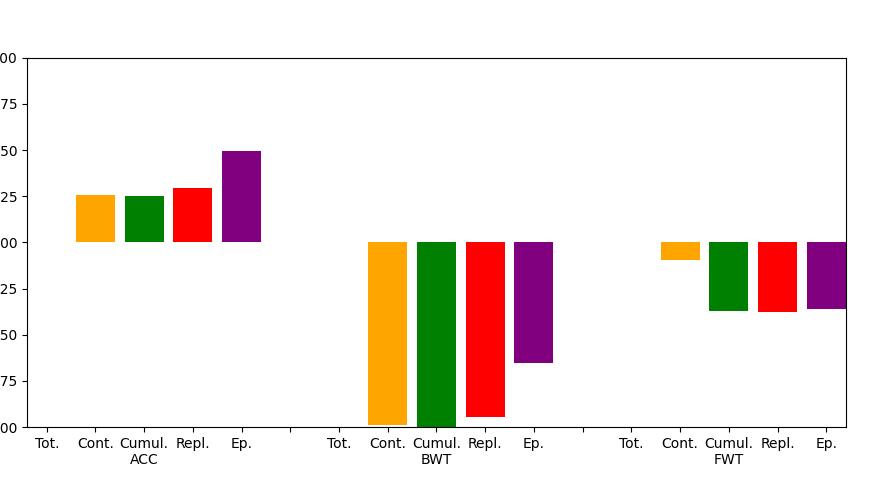
\includegraphics[scale=0.6]{img/autotest_20210701/autotest_task_GRU_accbwtfwt.png}
    \caption{Metriche task per task}
    \label{fig:autotest_task_GRU}
\end{figure}
\paragraph{Learning task per task} Di seguito\\
\begin{tabular}{l|c|c|c|c|c}
    \textbf{Scenario} & \textbf{Epoche} & \textbf{Accuracy} & \textbf{ACC} & \textbf{BWT} & \textbf{FWT} \\
    \hline 
    \textbf{Offline} & 18 & 53.24\% & - & - & - \\
    \textbf{Continual} & 99.25$\pm$1.3 & 26.47\%$\pm$15.68\% & 0.2570 & -0.9907 & -0.0935\\
    \textbf{Cumulative} & 99.25$\pm$1.3 & 32.64\%$\pm$17.07\% & 0.2507 & -0.9991 & -0.3695\\
    \textbf{Replay 25\%} & 99$\pm$1.73 & 31.24\%$\pm$11.05\% & 0.2918 & -0.9443 & -0.3756\\
    \textbf{$m = 70$} & 39.5$\pm$36.13 & \textbf{56.49\%$\pm$6.93\%} & 0.4938 & -0.6509 & -0.3595\\
\end{tabular}
\paragraph{Learning a coppie} Di seguito\\
\begin{tabular}{l|c|c|c|c|c}
    \textbf{Scenario} & \textbf{Epoche} & \textbf{Accuracy} & \textbf{ACC} & \textbf{BWT} & \textbf{FWT} \\
    \hline 
    \textbf{Offline} & 13 & 59.95\% & - & - & - \\
    \textbf{Continual} & 70$\pm$37.04 & 52.96\%$\pm$5.41\% & 0.4712 & -0.0042 & 0.0844\\
    \textbf{Cumulative} & 24.71$\pm$27.54 & 60.88\%$\pm$9.13\% & 0.4831 & -0.1369 & 0.3752\\
    \textbf{Replay 25\%} & 49.14$\pm$35.97 & \textbf{62.80\%$\pm$8.36\%} & 0.4942 & -0.0502 & 0.3903\\
    \textbf{$m = 70$} & 56.29$\pm$35.27 & 60.24\%$\pm$5.72\% & 0.4942 & -0.0502 & 0.3903\\
\end{tabular}
\subsection{Un po' di somme}
Partendo da un layer GRU da 29 unità seguito da un layer output Dense da 4 unità softmax, ho innanzitutto provato tre tecniche:
\begin{itemize}
    \item Total training: tutti i soggetti (escluso S17) sono stati uniti in un unico dataset e il modello è stato addestrato offline e testato su S17.
    \item Continual training: i soggetti sono stati divisi a coppie, escluso S17, e il modello è stato addestrato coppia per coppia testando su S17 dopo ogni coppia.
    \item Cumulative training: il training è stato eseguito coppia per coppia, ma le coppie precedentemente usate sono state mantenute anche nei training set successivi (quindi a con l'ultima coppia il training set equivaleva al dataset completo escluso S17)
\end{itemize}
Ho poi provato un modello con due layer GRU da 30 unità e un layer output Dense da 4 unità softmax sui primi due scenari di training, ottenendo fondamentalmente gli stessi risultati. Temendo overfitting, ho rifatto il dataset prendendo tutti i datapoint di ogni soggetto invece che solo una parte. Con quest'ultimo modello, sul dataset nuovo, ho ottenuto risultati migliori raggiungendo un 56\% di accuratezza sul training offline e un 53\% su quello continual.

Quindi ho provato un modello con due layer LSTM da 30 unità e un layer output Dense da 4 unità softmax, ottenendo risultati ancora migliori sui tre scenari. Ho aggiunto un nuovo scenario:
\begin{itemize}
    \item Replay training: dopo aver usato una coppia, ne mantengo il 25\% (default) dai dati da usare nel training assieme alla coppia successiva. Fornisce risultati a metà strada tra il continual e il cumulative.
\end{itemize}

Con la nuova tecnica, ho provato diversi modelli sia GRU che LSTM con un numero di unità tra i 30 e i 15. Ho concluso che il modello con un singolo layer LSTM da 30 unità e quello con un singolo layer GRU da 30 unità sono i migliori, procedendo a comparare le varie tecniche sul singolo layer GRU. Ottengo un comportamento del replay al 25\% comparabile al training offline, seppur oscillante tra l'85\% e il 55\% (con l'offline che si attesta sul 65\%). Il cumulative è molto più stabile, intorno al 60\% con una deviazione standard del 2\%.

Giudicando ottime le tecniche di replay, ne ho provate diverse:
\begin{itemize}
    \item Replay 10\%
    \item Replay 25\%
    \item Episodica  $m=50$  istanze
    \item Episodica  $m=50$  predizioni
\end{itemize}

Con il replay al 25\% e l'episodico sulle istanze con i comportamenti migliori. Ho provato anche con un layer LSTM da 30 unità e un layer output Dense da 4 unità softmax, ottenendo risultati simili ma migliori.

Ho confrontato i due modelli, ottenendo un risultato migliore su LSTM per il training offline, mentre le strategie continual si comportano meglio con GRU. Va però in contrasto con quanto osservato fin'ora.

Confrontando vari valori di  $m$, ho trovato in  $m=70$  il comportamento migliore. Andrebbe fatta un'altra ricerca in quell'intorno, magari tra 60 e 100.

Successivamente ho studiato diverse metriche (ACC, BWT e FWT) che confermano l'episodic come la tecnica migliore: finendo con un'ACC comparabile al replay al 10\%, ha però un catastrophic forgetting di quasi 10 volte inferiore.

Ho anche comparato l'apprendere task per task invece che coppia per coppia, ottenendo però accuratezze molto basse su continual, cumulative e replay, nonostante l'offline (dove il dataset non cambia) e l'episodic mantengano grossomodo le stesse capacità.

\begin{figure}[h]
    \centering
    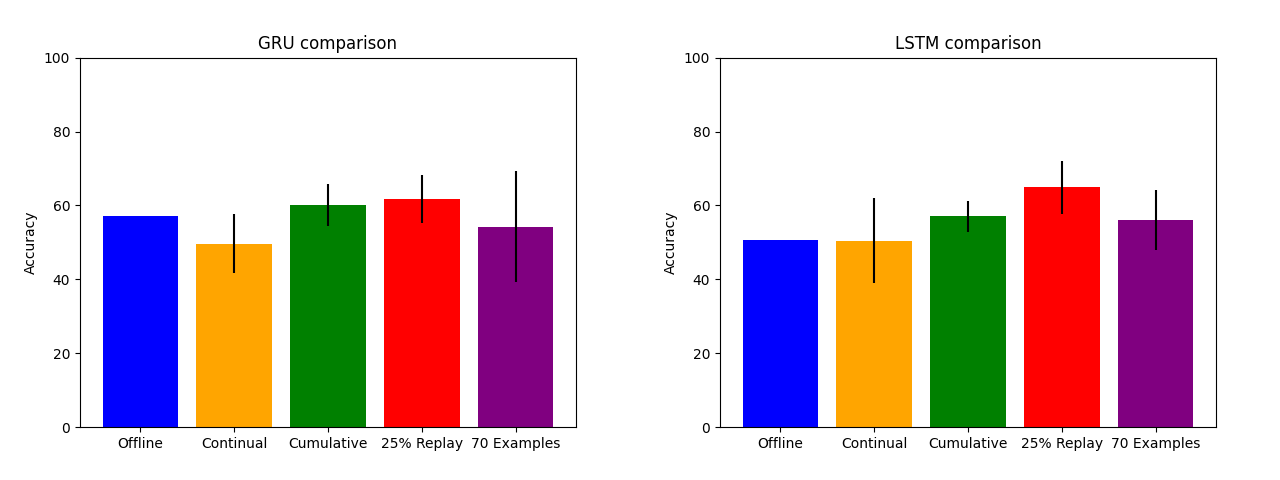
\includegraphics[scale=0.5]{img/autotestv.png}
    \caption{Comparazione fra modelli}
    \label{fig:autotest_comparison}
\end{figure}

\begin{figure}[h]
    \centering
    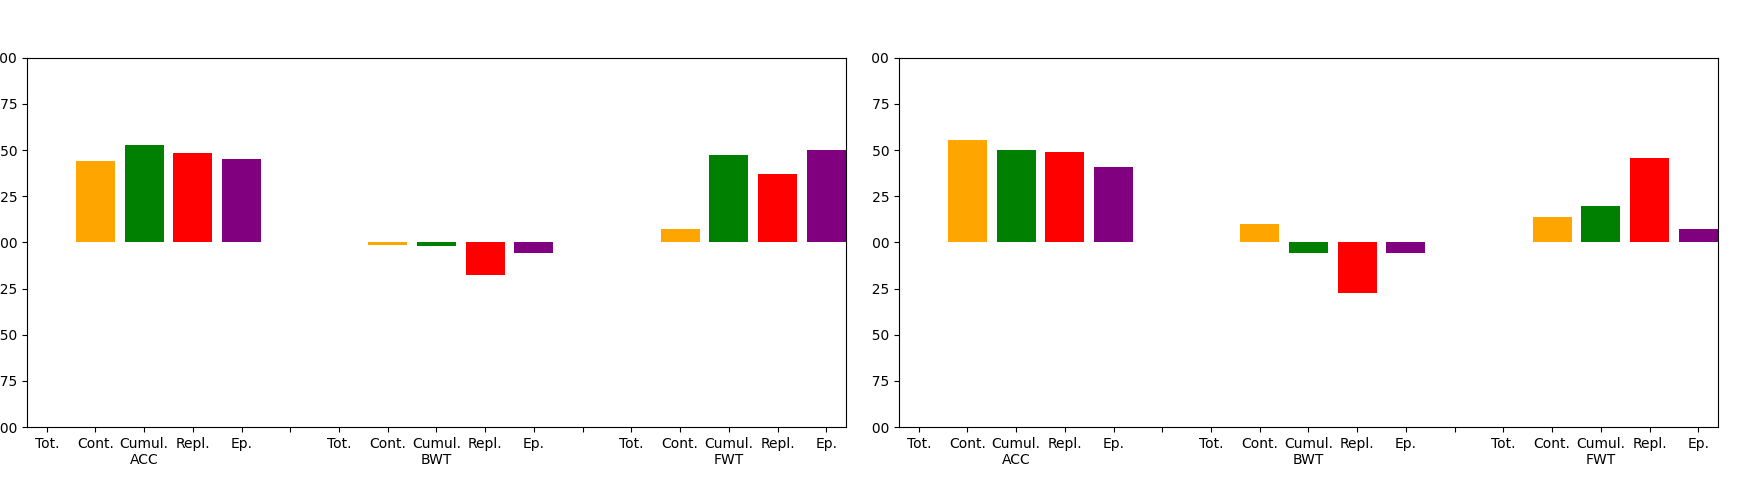
\includegraphics[scale=0.33]{img/autotestv_accbwtfwt.png}
    \caption{Comparazione fra modelli}
    \label{fig:autotest_comparison_metrics}
\end{figure}
\subsection{Tredicesimo test}
\paragraph{Generative replay} Ho valutato l'idea di creare un modello generativo per poter eseguire l'episodic training senza dover memorizzare i dati. L'idea che ho realizzato è molto semplice: allenare un modello "al contrario", cioè passandogli i label come input e aspettandomi come output le 14 features del dataset WESAD. L'ho realizzato con il seguente modello:
\begin{lstlisting}[language = Python]
model = tf.keras.models.Sequential()
model.add(tf.keras.layers.Dense(30))
model.add(tf.keras.layers.Dense(14,
                  kernel_regularizer = tf.keras.regularizers.l1_l2(l1 = 1e-6, l2 = 1e-6),
                  bias_regularizer = tf.keras.regularizers.l1_l2(l1 = 1e-4, l2 = 1e-4),
                  activity_regularizer = tf.keras.regularizers.l1_l2(l1 = 1e-4, l2 = 1e-4)))
opt = tf.keras.optimizers.Adam(learning_rate = 0.005, beta_1 = 0.85, beta_2 = 0.999)
model.compile(loss = 'mse', optimizer = opt)
\end{lstlisting}
Allenandolo sul dataset con batch da 512 elementi. Testandolo su S17 la loss è 0.9588 e testandolo velocemente, generando delle sequenze da 100 elementi per ogni classe, i risultati sono buoni:
\begin{lstlisting}[language = Python]
generator = tf.keras.models.load_model('wesad_generative.h5')
classificator = tf.keras.models.load_model('episodicGRU')
first, second, third, fourth = [], [], [], []
for i in range(100):
    first.append(generator.predict(np.array([[1., 0., 0., 0.]]))[0])
    second.append(generator.predict(np.array([[0., 1., 0., 0.]]))[0])
    third.append(generator.predict(np.array([[0., 0., 1., 0.]]))[0])
    fourth.append(generator.predict(np.array([[0., 0., 0., 1.]]))[0])

first = np.array(first).reshape(-1, 100, 14)
second = np.array(second).reshape(-1, 100, 14)
third = np.array(third).reshape(-1, 100, 14)
fourth = np.array(fourth).reshape(-1, 100, 14)

print(classificator.predict(first))
print(classificator.predict(second))
print(classificator.predict(third))
print(classificator.predict(fourth))
\end{lstlisting}
Output:
\begin{verbatim}
[[9.9999845e-01 5.4661302e-07 6.5005071e-07 2.8123785e-07]]
[[9.4253558e-08 9.9999928e-01 1.1999366e-07 4.3563784e-07]]
[[1.9276902e-06 1.3294758e-07 9.9997914e-01 1.8861941e-05]]
[[1.3735850e-07 1.3718072e-07 7.1482100e-07 9.9999905e-01]]
\end{verbatim}
Che dimostra come la generazione e il riconoscimento siano quantomeno sulla "stessa linea d'onda".
\paragraph{Scenario} Ho quindi prodotto uno script che ricalca quello dell'episodic learning ma genera $m$ sottosequenze invece di salvarne $m$ casuali dal dataset.\\
Provo due casi: uno dove genero i replay una sola volta, e li uso durante tutto il training, e uno dove li genero ad ogni coppia di utenti.
\paragraph{Risultati} A seconda di quando genero il replay set:\\
\begin{tabular}{l|c|c|c|c|c}
    \textbf{Generazione} & \textbf{Epoche} & \textbf{Accuracy} & \textbf{ACC} & \textbf{BWT} & \textbf{FWT} \\
    \hline 
    \textbf{A inizio training} & 76.29$\pm$37.95 & \textbf{55.76\%$\pm$9.56\%} & 0.5594 & -0.0482 & 0.2262 \\
    \textbf{Ad ogni coppia} & 61.14$\pm$44.95 & 52.95\%$\pm$11.34\% & 0.5646 & 0.0117 & -0.0240\\
\end{tabular}
\subsection{Quattordicesimo test}
Ho preparato il dataset ASCERTAIN e ho provato diversi modelli per selezionare quello con le performance migliori.
\paragraph{Risultati} Di seguito:\\
\begin{tabular}{l|c|c}
    \textbf{Modello} & \textbf{Epoche} & \textbf{Accuracy} \\
    \hline 
    \textbf{GRU 2 layer 16 unità} & 8 & 35.88\% \\
    \textbf{GRU 1 layer 24 unità} & 6 & 33.46\% \\
    \textbf{GRU 2 layer 24 unità} & 4 & \textbf{39.37\%} \\
    \textbf{LSTM 1 layer 40 unità} & 4 & 34.54\% \\
    \textbf{LSTM 1 layer 38 unità} & 5 & 35.32\% \\
    \textbf{LSTM 1 layer 35 unità} & 6 & 36.09\% \\
    \textbf{LSTM 1 layer 30 unità} & 4 & 35.32\% \\
    \textbf{LSTM 1 layer 20 unità} & 7 & 35.58\% \\
\end{tabular}\\
Il risultato è stato anche confermato da una gridsearch
\pagebreak
\subsection{Risultati test}
\paragraph{WESAD} Usando come modello un layer GRU da 30 unità, su WESAD ho ottenuto i seguenti risultati:

\begin{tabular}{l|c|c|c|c|c|c|c|c}
\textbf{Scenario} & \textbf{Epoche} & \textbf{Tempo} & \textbf{Tempo tot} & \textbf{Acc.} & \textbf{ACC} & \textbf{BWT} & \textbf{FWT} & \textbf{Memoria}\\
\hline
 \textbf{Offline} & 13 & 148,01s & 148,01 s & 54,68 & - & - & - & 2.391,51 Mb\\
\textbf{Continual} & 67,00$\pm$41,98 & 436,74 s & 3.057,18 s & 62,50$\pm$11,22 & 0,5988 & 0,1074 & 0,4392 & 2.189,70 Mb\\
\textbf{Cumulative} & 26,43$\pm$30,53 & 613,79 s & 4.296,53 s & \textbf{62,69$\pm$3,99} & 0,4825 & -0,041 & 0,4653 & 2.361,97 Mb\\
\textbf{Replay 25\%} & 57,29$\pm$35,93 & 479,29 s & 3.355,03 s & 57,52$\pm$9,62 & 0,4696 & -0,0526 & 0,3516 & 2.225,91 Mb\\
\textbf{m = 70} & 37,86$\pm$35,91 & 327,58 s & 2.293,06 s & 58,43$\pm$4,50 & 0,442 & -0,0868 & 0,2336 & 2.148,99 Mb\\
\textbf{EWC} & 71,57$\pm$41,46 & 878,08 s & 6.146,56 s & 56,80$\pm$9,66 & 0,4834 & -0,1785 & 0,2417 & 2.199,43 Mb\\
\textbf{LWF} & 73,86$\pm$33,39 & 2.601,09 s & 18.207,63 s & 50,41$\pm$9,94 & 0,4692 & -0,0393 & 0,1013 & 2.154,66 Mb\\
\end{tabular}
Usando come modello un layer LSTM da 30 unità, su WESAD ho ottenuto i seguenti risultati:

\begin{tabular}{l|c|c|c|c|c|c|c|c}
\textbf{Scenario} & \textbf{Epoche} & \textbf{Tempo} & \textbf{Tempo tot} & \textbf{Acc.} & \textbf{ACC} & \textbf{BWT} & \textbf{FWT} & \textbf{Memoria}\\
\hline
 \textbf{Offline} & 28 & 228.52 s & 228.52 s & \textbf{76.86} & - & - & - & 2.397,12 Mb\\
\textbf{Continual} & 62.86$\pm$43.37 & 436.59 s & 3.056,13 s & 54.11$\pm$9.91 & 0,4857 & 0,0002 & 0,0538 & 2.216,76 Mb\\
\textbf{Cumulative} & 12.86$\pm$9.09 & 557.89 s & 3905.23 s & 62.04$\pm$5.88 & 0,4914 & -0,128 & 0,3212 & 2404,07 Mb\\
\textbf{Replay 25\%} & 15.14$\pm$7.75 & 202.12 s & 1414.84 s & 57.55$\pm$4.13 & 0,4508 & -0,0961 & 0,1767 & 2208,65 Mb\\
\textbf{m = 70} & 29.29$\pm$30.47 & 257.25 s & 1800.75 s & 57.61$\pm$5.11 & 0,4821 & -0,2283 & 0,2044 & 2.146,38 Mb\\
\textbf{EWC} & 47.14$\pm$37.03 & 753.18 s & 5272.26 s & 53.49$\pm$9.31 & 0,4745 & 0,0121 & 0,3541 & 2195,50 Mb\\
\textbf{LWF} & 46.43$\pm$32.16 & 1699.19 s & 11894.33 s & 48.89$\pm$16.21 & 0,5276 & 0.0709 & -0,0287 & 2136,14 Mb\\
\end{tabular}
\paragraph{ASCERTAIN} Usando come modello due layer GRU da 24 unità, su ASCERTAIN ho ottenuto i seguenti risultati:

\begin{tabular}{l|c|c|c|c|c|c|c|c}
\textbf{Scenario} & \textbf{Epoche} & \textbf{Tempo} & \textbf{Tempo tot} & \textbf{Acc.} & \textbf{ACC} & \textbf{BWT} & \textbf{FWT} & \textbf{Memoria}\\
\hline
 \textbf{Offline} & 13 & 1.012,01 s & 1.012,01 s & 33,59 & - & - & - & 4.136,99 Mb\\
\textbf{Continual} & 7,38$\pm$2,50 & 680,06 s & 5.440,48 s & 34,50$\pm$4,87 & 0,2262 & 0,0747 & 0,0429 & 2.648,29 Mb\\
\textbf{Cumulative} & 7,5$\pm$7,19 & 3.171,71 s & 25.373,68 s & 	32,03$\pm$2,79 & 0,2781 & -0,0264 & 0,0346 & 4.066,37 Mb\\
\textbf{Replay 25\%} & 5,12$\pm$3,14 & 778,39 s & 6.227,12 s & 33,99$\pm$4,36 & 0,202 & -0,0434 & 0,0465 & 2.732,64 Mb\\
\textbf{m = 70} & 5,12$\pm$2,71 & 647,57 s & 5.180,56 s & 35,00$\pm$4,16 & 0,2404 & 0,0569 & -0,038 & 2.815,67 Mb\\
\textbf{EWC} & 18,88$\pm$9,58 & 2.583,83 s & 20.670,64 s & \textbf{35,41$\pm$3,48} & 0,2425 & -0,0593 & 0,051 & 2.497,26 Mb\\
\textbf{LWF} & 13,88$\pm$1,54 & 2.199,38 s & 17.595,04 s & 35,21$\pm$3,83 & 0,2556 & 0,0551 & 0,0413 & 2.369,36 Mb\\
\end{tabular}
Usando come modello un layer LSTM da 35 unità, su ASCERTAIN ho ottenuto i seguenti risultati:

\begin{tabular}{l|c|c|c|c|c|c|c|c}
\textbf{Scenario} & \textbf{Epoche} & \textbf{Tempo} & \textbf{Tempo tot} & \textbf{Acc.} & \textbf{ACC} & \textbf{BWT} & \textbf{FWT} & \textbf{Memoria}\\
\hline
 \textbf{Offline} & 5 & 390.34 s & 390.34 s & \textbf{37.95} & - & - & - & 4115.21 Mb\\
\textbf{Continual} & 5.75$\pm$2.68 & 386.83 s & 3094.64 s & 34,97$\pm$4,50 & 0,2298 & 0,0677 & -0,027 & 2567.67 Mb\\
\textbf{Cumulative} & 4$\pm$2.45 & 1425.36 s & 11402.88 s & 31.15$\pm$2.54 & 0,2484 & -0,0057 & 0,0525 & 3566.31 Mb\\
\textbf{Replay 25\%} & 4.62$\pm$4.09 & 485.86 s & 3886.88 s & 34.23$\pm$4.57 & 0,207 & 0,0341 & -0,0526 & 2556.10 Mb\\
\textbf{m = 70} & 5.88$\pm$3.06 & 434.11 s & 3472.88 s & 33.70$\pm$4.02 & 0,210 & 0,0467 & 0,0103 & 2724.39 Mb\\
\textbf{EWC} & 18.88$\pm$15.02 & 1660.97 s & 13287.76 s & 33.86$\pm$4.48 & 0.2404 & 0.0608 & 0.0315 & 2551.47 Mb\\
\textbf{LWF} & 17$\pm$2.92 & 1952.19 s & 15617.52 s & 34.31$\pm$3.43 & 0.2334 & 0.0557 & 0.0017 & 2684.69 Mb\\
\end{tabular}
\section{Altre strategie}
\subsection{Elastic Weight Consolidation}
L'implementazione è stata fatta seguendo questo codice\\ \texttt{https://seanmoriarity.com/2020/10/18/continual-learning-with-ewc/}
aggiungendo un output più descrittivo, l'early stopping (con patience = 10) e adattando il training loop per essere eseguito mentre arrivano le coppie di soggetti. Il file in questione è \texttt{ewc\_train.py} al seguente link\\ \texttt{https://teaching-gitlab.di.unipi.it/f.matteoni/thesis-code/-/blob/master/ewc\_train.py}
\begin{tabular}{l|c|c|c|c|c}
    \textbf{Dataset} & \textbf{Epoche} & \textbf{Accuracy} & \textbf{ACC} & \textbf{BWT} & \textbf{FWT} \\
    \hline 
    \textbf{WESAD} & 58$\pm$43.38 & 50.13\%$\pm$12.61\% & 0.3646 & -0.195 & 0.1902\\
    \textbf{ASCERTAIN} & 28.88$\pm$14.72 & 34.70\%$\pm$3.98\% & 0,2327 & 0,0473 & -0,0206
\end{tabular}
\subsection{Learning Without Forgetting}
L'implementazione è stata realizzata seguendo il paper relativo, al link\\ \texttt{https://arxiv.org/pdf/1606.09282.pdf}. Anche qua, aggiungendo un output più descrittivo, l'early stopping (con patience = 10) e adattando il training loop per essere eseguito mentre arrivano le coppie di soggetti. Il file in questione è \texttt{lwf\_train.py} al seguente link\\ \texttt{https://teaching-gitlab.di.unipi.it/f.matteoni/thesis-code/-/blob/master/lwf\_train.py}
\begin{tabular}{l|c|c|c|c|c}
    \textbf{Dataset} & \textbf{Epoche} & \textbf{Accuracy} & \textbf{ACC} & \textbf{BWT} & \textbf{FWT} \\
    \hline 
    \textbf{WESAD} & 86.71$\pm$21.61 & 55.7\%$\pm$11.20\% & 0.5585 & 0.0722 & -0.1078\\
    \textbf{ASCERTAIN} & 13.5$\pm$1.41 & 34,77\%$\pm$4,01\%& 0,2077 & 0,0278 & -0,0316
\end{tabular}

\section{Problema nell'accuracy}
Facendo un veloce recap, fino alla call con Lomonaco di Mercoledì io usavo l’intero dataset WESAD, diviso per soggetti, mentre da Mercoledì ho provato a bilanciarlo prendendo, per ogni soggetto, 100 sequenze da 100 datapoint per ogni classe così da mitigare lo sbilanciamento delle classi. Da allora ho cercato un modello che mi garantisse un’accuracy offline apprezzabile, ma non sono mai andato sopra il 50\% (con qualche falso positivo che ha dato il 70\% circa).\\
La differenza fondamentale che ho notato rispetto al paper di riferimento (RNN for HSM) è che io uso come test set S17, poiché nello scenario continual avendo soggetto per soggetto ho pensato che il “test” più sensato sia classificare i dati del soggetto in arrivo, mentre nel paper viene usata la classica partizione del dataset comprensivo di tutti i soggetti. Così facendo, anche io riesco ad ottenere un’accuracy intorno al 95\%.\\\\
La mia conclusione è che la difficoltà sta nel classificare i dati di un solo soggetto invece di prendere dati dai soggetti precedenti. Mi spiego meglio: se uso solo S17 come soggetto di test, e il training lo eseguo sui soggetti precedenti, non riesco a classificare bene S17 perché è una persona nuova, diversa, con parametri diversi per le classi.

\paragraph{WESAD} La soluzione consiste nel creare un test set estraendo dati da ogni soggetto, e mantenere i soggetti separati senza però i dati che sono stati selezionati nel test set.\\
Così facendo, dopo un po' di prove, ottengo un modello che raggiunge il 99.40\% di accuracy sul test set "partizionato".

\paragraph{ASCERTAIN} Per ASCERTAIN ho scelto un approccio diverso: i soggetti sono stati tutti "uniti" per poi essere risuddivisi in soggetti fittizi con un migliore bilanciamento delle classi.

\subsection{Risultati finali}
\paragraph{WESAD} Usando come modello due layer GRU da 18 unità, su WESAD ho ottenuto i seguenti risultati:\\
\begin{tabular}{l|c|c|c|c|c|c|c}
\textbf{Scenario} & \textbf{Epoche} & \textbf{Tempo tot} & \textbf{Acc.} & \textbf{ACC} & \textbf{BWT} & \textbf{FWT} & \textbf{Memoria}\\
\hline
 \textbf{Offline} & 28 & 94,69 s & 99,07 & - & - & - & 2061,40 Mb\\
\textbf{Continual} & 54$\pm$38,53 & 1044,89 s & 74,09$\pm$2,05 & 0,7829 & 0,0377 & 0,4181 & 2169,16 Mb\\
\textbf{Cumulative} & 39$\pm$19,35 & 3160,43 s & 83,75$\pm$7,38 & 0,8323 & 0,0248 & 0,06989 & 2293,87 Mb\\
\textbf{Replay 25\%} & 40,14$\pm$28,26 & 1071,70 s & 78,51$\pm$6,92 & 0,8236 & 0,0483 & 0,4870 & 2184,77 Mb\\
\textbf{m = 70} & 24,43$\pm$23,27 & 817,18 s & 78,92$\pm$7,89 & 0,8912 & 0,086 & 0,3796 & 2105,37 Mb\\
\textbf{EWC} & 43,14$\pm$22,82 & 500,08 s & 71,44$\pm$5,02 & 0,7738 & 0,1154 & 0,504 & 2192,25 Mb\\
\textbf{LWF} & 40,57$\pm$14,29 & 3308,34 s & 70,27$\pm$2,99 & 0,7125 & 0,0966 & 0,4063 & 2127,07 Mb\\
\end{tabular}

\paragraph{ASCERTAIN} Usando come modello due layer GRU da 24 unità, su ASCERTAIN ho ottenuto i seguenti risultati:\\
\begin{tabular}{l|c|c|c|c|c|c|c}
\textbf{Scenario} & \textbf{Epoche} & \textbf{Tempo tot} & \textbf{Acc.} & \textbf{ACC} & \textbf{BWT} & \textbf{FWT} & \textbf{Memoria}\\
\hline
 \textbf{Offline} & 3 & 29,14 s & 42,78 & - & - & - & 1817,28 Mb\\
\textbf{Continual} & 23$\pm$13,77 & 408,48 s & 37,90$\pm$4,65 & 0,2532 & 0,0735 & -0,119 & 2166,97 Mb\\
\textbf{Cumulative} & 8,62$\pm$8,03 & 961.04 s & 38,77$\pm$4,97 & 0,2843 & -0,0362 & -0,0558 & 2293,38 Mb\\
\textbf{Replay 25\%} & 10,38$\pm$13,36 & 330 s & 39,06$\pm$4.10 & 0,2675 & 0,1315 & -0,0755 & 2172,41 Mb\\
\textbf{m = 70} & 8,88$\pm$6,21 & 446,64 s & 36,89$\pm$6,31 & 0,2844 & -0,019 & 0,2685 & 2225,02 Mb\\
\textbf{EWC} & 25,12$\pm$14,35 & 836,16 s & 36,30$\pm$4,50 & 0,2256 & -0,0309 & 0,0984 & 2168,57 Mb\\
\textbf{LWF} & 24,62$\pm$16,73 & 942 s & 37,64$\pm$5,45 & 0,2601 & 0.0837 & 0,1088 & 2113,61 Mb\\
\end{tabular}
\fi
\end{document}